    %\documentclass[sigconf,review,anonymous, table]{acmart} 
\documentclass[manuscript,review,screen, table]{acmart}
%\documentclass[sigconf,anonymous, table]{acmart}
\usepackage{paralist}
% \usepackage{enumitem,kantlipsum}
\usepackage{enumitem}
\usepackage{pgf-pie}
\usepackage{tikz}
\usepackage[most]{tcolorbox}
\usepackage{etoolbox}
\usepackage{fp}
\usepackage{subcaption}
\usepackage{mwe}
\usepackage{xspace}
\usepackage{eurosym}
\usepackage{mdframed,ifthen}
\usepackage{array}
\tcbuselibrary{listings,breakable}
\usepackage{placeins,newfloat}
\usepackage{booktabs}
\usepackage[multiple]{footmisc}

\def\bf{\textbf}
\def\eq {Equation~}
\def\eqm {Eq~}
\def\eqs {Equations~}
\def\fig {Figure~}
\def\figs {Figures~}
\def\tbl {Table~}
\def\tbls {Tables~}
\def\ie{\textit{i.e.,}}
\def\eg{\textit{e.g.,}}
\def\sec {Section~}
\def\secs {Sections~}
\def\alg {Algorithm~}
\def\algs {Algorithms~}
\def\app {Appendix~}
\def\it{\textit}
\def\tr{\textrm}
\def\tt{\mct}
%\newcommand{\ib}[1]{{\textbf {\textit { #1}}}}
%\newcommand{\ts}[1]{{\textsc {{ #1}}}}
\newcommand{\mct}[1]{{\footnotesize {\texttt {#1}}}}

\newcommand{\qu}[1]{{\it{``#1''}}}
\newcommand{\api}[1]{{\sf{\texttt\small{#1}}}}
\newcommand{\callout}[1]{{\vspace{1mm}\noindent{\fbox{\parbox{0.97\columnwidth}{#1}}}\vspace{1mm}}}
\usepackage{paralist}
\usepackage{hyperref}
\usepackage{soul}


%% We use a different version in the main paper and in appendix!
\newenvironment{practice}[2]
    {
   \begin{center}\begin{tcolorbox}[%width=.48\textwidth, 
   %breaking, 
   skin=enhanced jigsaw, arc=0pt, title={\textbf{Decision Pattern #1: #2}}]
    
    }
    {\end{tcolorbox}\end{center} }

%    \DeclareFloatingEnvironment[fileext=frm,placement={!ht},name=Frame]{nonIncrementingFloat}
%\newenvironment{practice}[2]
 %   {
 %       \begin{center}
 %       \begin{nonIncrementingFloat}
 %       \begin{tcolorbox}[width=.48\textwidth, skin=enhanced jigsaw, breakable, arc=0pt, title={\textbf{Guiding Principle #1: #2}}]}
%    {\end{tcolorbox}\end{nonIncrementingFloat}\end{center}
%    }


\normalsize
\let\labelindent\relax
% \usepackage{enumitem}

\newcommand{\nd}{\vspace{1mm}\noindent}
\usepackage{caption}
%\usepackage[toc,page]{appendix}
\usepackage{tikz}
\newcommand*\circled[1]{\tikz[baseline=(char.base)]{
            \node[shape=circle,draw,inner sep=1pt] (char) {#1};}}

 \lstset{
         language=Java,
         basicstyle=\scriptsize\ttfamily, % Standardschrift
         %numbers=left,               % Ort der Zeilennummern
         numberstyle=\tiny,          % Stil der Zeilennummern
         %stepnumber=2,               % Abstand zwischen den Zeilennummern
         numbersep=5pt,              % Abstand der Nummern zum Text
         tabsize=2,                  % Groesse von Tabs
        % extendedchars=true,         %
         breaklines=true,            % Zeilen werden Umgebrochen
%         keywordstyle=\color{black},
 %   	 frame=single,
 %        keywordstyle=[1]\textbf,    % Stil der Keywords
 %        keywordstyle=[2]\textbf,    %
 %        keywordstyle=[3]\textbf,    %
 %        keywordstyle=[4]\textbf,   \sqrt{\sqrt{}} %
         stringstyle=\color{white}\ttfamily, % Farbe der String
         showspaces=false,           % Leerzeichen anzeigen ?
         showtabs=false,             % Tabs anzeigen ?
         xleftmargin=17pt,
         framexleftmargin=17pt,
         framexrightmargin=5pt,
         framexbottommargin=4pt,
         %backgroundcolor=\color{lightgray},
         showstringspaces=false,      % Leerzeichen in Strings anzeigen ?
     %    escapeinside={\%*}{*)}
 }
\usepackage{rotating}
\usepackage{pdflscape}
\lstdefinestyle{inlinecode}{basicstyle={\ttfamily\scriptsize\bfseries}}
%\newcommand\code{\lstinline[style=inlinecode]}
%\newcommand{\urls}[1]{{\scriptsize\url{#1}}}
\usepackage{tcolorbox}
\newcommand{\emt}[1]{\emph{``#1''}}
\usepackage{paralist}
\usepackage[outercaption]{sidecap}    
%\usepackage{unicode-math}
%\usepackage{amssymb}% http://ctan.org/pkg/amssymb
\usepackage{pifont}% http://ctan.org/pkg/pifont
\newcommand{\cmark}{\ding{51}}%
\newcommand{\xmark}{\ding{55}}%

\newcommand{\dc}[1]{\href{https://devrant.com/rants/#1/}{$R_{#1}$}}
\usepackage{soul}
% \usepackage{enumitem}
\hypersetup{
    colorlinks=true,
    linkcolor=blue,
    filecolor=magenta,      
    urlcolor=cyan,
}
\newtcolorbox
{mybox}[2][]{colbacktitle=red!10!white,
colback=blue!10!white,coltitle=black!70!black,
title={#2},fonttitle=\bfseries,#1}

\usepackage{xcolor}
\definecolor{ao(english)}{rgb}{0.0, 0.5, 0.0}
\newcommand{\mybars}[3]{
  {\color{red}\rule{#1pt}{6pt}}
  {\color{yellow}\rule{#2pt}{6pt}}
  {\color{ao(english)}\rule{#3pt}{6pt}}
}
\newcommand{\mybarsbwv}[3]{
  {#1\%\color{black!90}\rule{#1pt}{6pt}}
  {#2\%\color{black!50}\rule{#2pt}{6pt}}
  {#3\%\color{black!20}\rule{#3pt}{6pt}}
}
\newcommand{\mybarsbw}[3]{
  {\color{black!90}\rule{#1pt}{6pt}}
  {\color{black!50}\rule{#2pt}{6pt}}
  {\color{black!20}\rule{#3pt}{6pt}}
}
\newcommand{\mybarsbwa}[3]{
  {#1\%Negative~\color{black!90}\rule{#1pt}{6pt}}\\
  {#2\%Neutral~\color{black!50}\rule{#2pt}{6pt}}\\
  {#3\%Positive~\color{black!20}\rule{#3pt}{6pt}}
}

%\newcommand{\rev}[1]{\textcolor{blue}{ #1}}
\newcommand{\rev}[1]{#1}
\newcommand{\newrev}[1]{\textcolor{blue}{ #1}}
\newcommand{\as}[1]{{\textcolor{magenta}{\sf{\texttt\small{#1}}}}}

\newcommand{\code}[1]{{\fontfamily{lmdh}\selectfont{\small\textsl{#1}}\normalfont}} 
\newcommand{\ab}[1]{{\color{red}{Ann: #1}}}
\newcommand{\numInterviews}{24\xspace}
\newcommand{\todo}[1]{{\color{red}{\textbf{#1}}}}

 %% Ann: I hate the way \qw looks so I've replaced \qw with this new command, \qqw. If the consensus is to return to the look of \qw, this command can be redefined.
 % \newcommand{\qqw}[2]{{{\fontfamily{lmdh}\selectfont{\small\textsl{#2}}\normalfont}} (#1)\xspace} %% Usage: \qqw{F}{stability}
  \newcommand{\qqw}[2]{{{\fontfamily{lmdh}\selectfont{\small\textsl{#2}}\normalfont}}\xspace} %% Usage: \qqw{F}{stability}
 \newcommand{\qww}[1]{(#1)\xspace} %% Usage: \qww{F}



\newcommand{\gias}[1]{\textcolor{red}{{[Gias: #1]}}}

% Used to format quotations. Usage:
% Attributed quote: \quotebox{P4}{That's annoying.}
% Unattributed quote: \quotebox{}{I've heard the comment.}
\newenvironment{smallquote}%
{\list{}{\leftmargin=0.15in\rightmargin=0.15in}\item[]}%
  {\endlist}
  
\newcommand{\quotebox}[2]{\begin{smallquote}\textit{``#2''}\ifthenelse{\equal{#1}{}}{}{ \mbox{-}~#1}\end{smallquote}}

\newenvironment{observation}[2]{
        \begin{mdframed}[
                frametitle={\colorbox{white}{\space #1}},
                innertopmargin=0pt,
                frametitleaboveskip=-\ht\strutbox,
                frametitlealignment=\raggedright,
                nobreak=true,
                skipabove=10pt,
                skipbelow=10pt,
        ]%
        \label{#2}}{\end{mdframed}}



\newcounter{recommendation}[section]
\renewcommand{\therecommendation}{\arabic{recommendation}}

\newenvironment{recommendation}[1]{
        %\refstepcounter{observation}
        \addtocounter{recommendation}{1}
        \begin{mdframed}[
                frametitle={\colorbox{white}{\space Recommendation \therecommendation\space}},
                innertopmargin=0pt,
                frametitleaboveskip=-\ht\strutbox,
                frametitlealignment=\raggedright,
                nobreak=true,
%                skipabove=10pt,
                skipbelow=10pt,
        ]%
        \label{#1}}{\end{mdframed}}

%\mdfsetup{skipabove=\topskip,skipbelow=\topskip}
\mdfsetup{skipabove=2,skipbelow=5}

\def\nonzero#1#2{%
    \ifnum #1 > 0
      #1#2
    \fi
}


% \newcommand{\horizontalbars}[4]{
% {{\color{black}\rule{#1pt}{4pt}}  \nonzero{#1}{C}}
% {{\color{black!50}\rule{#2pt}{4pt}}  \nonzero{#2}{F}}
% {{\color{black!20}\rule{#3pt}{4pt}}  \nonzero{#3}{P}}
% {{\color{black!40}\rule{#4pt}{4pt}} \nonzero{#4}{S}}

% }

% \newcommand{\horizontalbars}[5]{
% {{\color{black}\rule{#1pt}{4pt}}  \nonzero{#1}{NA}}
% {{\color{red}\rule{#2pt}{4pt}}  \nonzero{#2}{AS}}
% {{\color{green}\rule{#3pt}{4pt}}  \nonzero{#3}{EU}}
% {{\color{blue}\rule{#4pt}{4pt}} \nonzero{#4}{AU}}
% {{\color{black!50}\rule{#5pt}{4pt}} \nonzero{#5}{SA}}
% }


\newcommand{\horizontalbars}[5]{
{{\color{black}\rule{\fpeval{5*(#1)}pt}{4pt}}\nonzero{#1}{}}{{\color{red}\rule{\fpeval{5*(#2)}pt}{4pt}}\nonzero{#2}{}}{{\color{green}\rule{\fpeval{5*(#3)}pt}{4pt}}\nonzero{#3}{}}{{\color{blue}\rule{\fpeval{5*(#4)}pt}{4pt}}\nonzero{#4}{}}{{\color{black!50}\rule{\fpeval{5*(#5)}pt}{4pt}}\nonzero{#5}{}}
}

%\newcommand{\mybarsbwa}[4]{}
% \\   {C\color{black!90}\rule{#1pt}{6pt}}#1 {P\color{black!70}\rule{#2pt}{6pt}}#2 {F\color{black!40}\rule{#3pt}{6pt}}#3 {S\color{black!20}\rule{#4pt}{6pt}}#4
% }


%\newcommand{\qq}[2]{} % remove all quotes
%\newcommand{\qq}[2]{\textit{"#1"}$_{#2}$} % inline quotes
%\newcommand{\qi}[2]{\textit{"#1"}$_{#2}$} % inline quotes
%\newcommand{\qq}[2]{\begin{quote}"#1"$_{#2}$\end{quote}} % stylized quotes

\newcommand{\qi}[2]{\quotebox{#2}{#1}}
\newcommand{\qq}[2]{\quotebox{#2}{#1}} 
\newcommand{\qqi}[2]{\textit{"#1"} - {#2}} % inline quotes




%This is an apple {\def\svgwidth{2cm}\input{name.pdf_tex}} and more text
%https://tex.stackexchange.com/questions/374192/how-to-use-figures-as-inline-images
%https://tex.stackexchange.com/questions/313927/tikz-picture-inline
%https://tex.stackexchange.com/questions/7032/good-way-to-make-textcircled-numbers
\newcommand{\qw}[2]{\textbf{#2}\tikz[baseline=(char.base)]{
    \node[shape=circle,fill=blue!20,inner sep=.5pt] (char){#1};}}

\newcommand{\tc}[0]{\textcolor{green}{ [add citation]}}

% following command is used to highlight text/numbers which can be changed after all the inerview/data collection is done. 
\newcommand{\td}[1]{\textcolor{blue}{(#1)}}

\newcommand{\autourfill}[1]{\tikz[baseline=(X.base)]\node [draw=blue,fill=blue!40,semithick,rectangle,inner sep=2pt, rounded corners=3pt] (X) {#1};}

\newcommand{\autouroutline}[1]{\tikz[baseline=(X.base)]\node [draw=blue,fill=white,semithick,rectangle,inner sep=2pt, rounded corners=3pt] (X) {#1};}

\newcommand{\autourbox}[1]{\tikz[baseline=(X.base)]\node [draw=black!70,fill=white,semithick,rectangle,inner sep=2pt, rounded corners=3pt] (X) {#1};}

\newcommand{\autourhighlight}[1]{\tikz[baseline=(X.base)]\node [draw=none,fill=red!20,semithick,rectangle,inner sep=2pt, rounded corners=3pt](X){#1};}




\newcommand\actor[1]{\textbf{Actor:}  #1\vspace*{.5em}\\} 
\newcommand\condition[1]{\textbf{Condition:}  #1\vspace*{.5em}\\} 
\newcommand\concern[1]{\textbf{Concern:} #1\vspace*{.5em}\\}
\newcommand\solution[1]{\textbf{Solution:} #1\vspace*{.5em}\\ }
\newcommand\consideration[1]{ \textbf{Consideration:} #1 }
\newcommand\steps[1]{\vspace*{.5em}\\\textbf{Steps:} #1}
\newcommand\example[2]{\vspace*{.5em}\\\textbf{Example Data:} \qqi{#1}{#2}}

%\newcommand{minaoar}[1]{\textcolor{blue}{Minaoar: #1}}

%\newcommand\minaoar[1]{\textcolor{blue}{#1}}
\newcommand{\minaoar}[1]{\textcolor{blue}{{[Minaoar]: #1}}}

  \setlength\heavyrulewidth{0.30ex}
  \setlength\cmidrulewidth{0.10ex}
  \setlength\lightrulewidth{0.10ex}
\AtBeginDocument{%
  \providecommand\BibTeX{{%
    \normalfont B\kern-0.5em{\scshape i\kern-0.25em b}\kern-0.8em\TeX}}}

\setcopyright{acmcopyright}
\copyrightyear{2023}
\acmYear{2023}
\acmDOI{XXXXXXX.XXXXXXX}

%% These commands are for a PROCEEDINGS abstract or paper.
%\acmConference[ESEC/FSE 2023]{The 31st ACM Joint European Software Engineering Conference and Symposium on the Foundations of Software Engineering}{11 - 17 November, 2023}{San Francisco, USA}

%
%  Uncomment \acmBooktitle if th title of the proceedings is different
%  from ``Proceedings of ...''!
%
%\acmBooktitle{Woodstock '18: ACM Symposium on Neural Gaze Detection,
%  June 03--05, 2018, Woodstock, NY} 
\acmPrice{15.00}
\acmISBN{978-1-4503-XXXX-X/18/06}

\begin{document}
%\title{Library Consumer Behavior Model: Challenges and Tools for Library Adoption}
%\title{A Theory of Software Library Adoption Model}
\title[The Promises and Perils of Third-Party API Selection]{\textit{``How do people decide? There are like 50 things implementing the same thing. Which one should I use?"}: The Promises and Perils of Third-Party API Selection}
%\title{Process, Factors, Conditions and Guiding Principles: A Model of Software Library Adoption in %Industry}

% \title{Guiding Principles for the Software Library Adoption Process: Perspectives from Industry}

%\title{A Model of Software Library Adoption in the Industry}

%\title{Promises and Perils of the Software Library Adoption Process}
%\title{Processes and Principles Guiding Software Library Adoption in the Industry: Perspectives from Industrial Developers}
%\title{The Process and Principles of Software Library Adoption: Perspectives from Industrial Developers}

%\title{How Industrial Developers Compare \& Adopt Software Libraries}
%\title{To Buy or Not to Buy: How Developers Buy Third-Party Libraries}
%\title{Third-Party Libraries: Reusable Wheel that Requires Continuous Tire Pressure Monitoring}
%\title{Choosing Third-Party Libraries: A Common Necessity with Maintenance Baggage}
%\title{Choosing Third-Party Libraries: A Vehicle with Risk of Brake Failure}

\author{Minaoar Tanzil}
%\authornote{Both authors contributed equally to this research.}
\email{minaoar.tanzil@ucalgary.ca}
%\orcid{1234-5678-9012}
\author{Gias Uddin}
%\authornotemark[1]
\email{gias.uddin@ucalgary.ca}
\author{Ann Barcomb}
%\authornotemark[1]
\email{ann.barcomb@ucalgary.ca}
\affiliation{%
  \institution{University of Calgary}
  \streetaddress{P.O. Box 1212}
  \city{Calgary}
  \state{Alberta}
  \country{Canada}
  \postcode{T2N 1N4}
}


%%
%% By default, the full list of authors will be used in the page
%% headers. Often, this list is too long, and will overlap
%% other information printed in the page headers. This command allows
%% the author to define a more concise list
%% of authors' names for this purpose.
\renewcommand{\shortauthors}{Tanzil et al.}

%%
%% The abstract is a short summary of the work to be presented in the
%% article.
\begin{abstract}
Modern-day rapid software development is often facilitated by the reuse of third-party software libraries. Software library adoption includes the selection as well as the maintenance of a library. Various factors and conditions may influence the adoption of a software library in a company. However, while literature offers insights on what factors could influence the selection of a library, we are not aware of any study that offers insights into the overall process and {\principle} that companies follow to adopt a software library. In this paper, we explore how the conditions and factors of the environment influence developer decisions in library selection. Using Straussian grounded theory, we conducted \numInterviews semi-structured interviews. The result is a theoretical framework of a \model, six \principle\space of library adoption, and seven barriers faced by developers and organizations. Inspired by the model, we proposed and evaluated two conceptual library selection tools. Our work lays the groundwork for the development of an industry-grade comparative library analysis tool to enable efficient decisions about libraries.
%consisting of 5 steps, 5 major information sources, 53 selection factors and conditions and 6 overarching guiding principles. The library adoption model can be used for the development of a comparative library analysis tool to enable faster and more accurate decisions among developers.
\end{abstract}

%%
%% The code below is generated by the tool at http://dl.acm.org/ccs.cfm.
%% Please copy and paste the code instead of the example below.
%%
% \begin{CCSXML}
% <ccs2012>
%    <concept>
%        <concept_id>10011007.10011006.10011072</concept_id>
%        <concept_desc>Software and its engineering~Software libraries and repositories</concept_desc>
%        <concept_significance>500</concept_significance>
%        </concept>
%    <concept>
%        <concept_id>10003120.10003130.10011762</concept_id>
%        <concept_desc>Human-centered computing~Empirical studies in collaborative and social computing</concept_desc>
%        <concept_significance>300</concept_significance>
%        </concept>
%  </ccs2012>
% \end{CCSXML}

\ccsdesc[500]{Software and its engineering~Software libraries and repositories}
\ccsdesc[300]{Human-centered computing~Empirical studies in collaborative and social computing}

%%
%% Keywords. The author(s) should pick words that accurately describe
%% the work being presented. Separate the keywords with commas.
\keywords{third-party, software library, adoption process, decision pattern, open-source software, grounded theory, interview study, qualitative research} % AB: added last 2 terms as these were present in my recent ICSE paper, added OSS because we mention it a lot and most of my research has this tag, added pattern because we do use that format and that's another large community
%%
%% This command processes the author and affiliation and title
%% information and builds the first part of the formatted document.
\maketitle
%\balance
\section{Introduction}
In 2011, Marc Andersson famously noted that \textit{"Software is eating the world"} \cite{website:eat-world}. Indeed, software has now become the enabler of almost every task we do or service we offer/consume. With growing demands for tools and techniques, software companies seek to build and deploy their products quickly and efficiently. Modern-day rapid software development is often facilitated by the reuse of third-party software libraries or APIs (Application Programming Interfaces). The libraries can be open-source or proprietary. Nevertheless, software/IT companies benefit from the adoption of third-party software libraries and often prefer the reuse of a library over the re-implementation of a feature from scratch~\cite{uddin2017opiner}. For example, according to a 2017 report by the European Commission, the use of open-source software saves European companies approximately \euro456 billion per year through increased productivity, efficiency, and direct cost savings \cite{eu2017economic}. These advantages come from standardization and reductions in vulnerability, development time, and required expertise. However, such benefits do not always accrue; Spinellis outlines many potential concerns of relying on an open-source library, among them: the project might not be maintained, the code may not be of high quality, the license may not allow the desired use, and the documentation may be poor \cite{spinellis2019select}.

The process of selecting a library is not simple, as it requires balancing a number of considerations, both those inherent to the library itself and those relating to the context in which it will be used. Developers or the deciding team in a company must ask questions like whether the library will accommodate the company's expansion plans and what the full legal implications are of using the library (including potentially hidden obligations) 
\cite{spinellis2019select,wolter:2022:open}. Factors such as the fit between the functional capability of available software and the acceptance (or rejection) of the technology by peers may also influence the selection decision \cite{dishaw1998supporting,eckhardt2009influences}. % Dishaw: Fit is the matching of the capabilities of the tech- nology to the demands of the task.

While open-source software represents a large proportion of the external libraries, companies also routinely use proprietary libraries \cite{harutyunyan:2018:understanding}. All of the considerations of open source software still apply: the company needs to consider if the library will continue to be developed, is a good fit for the task, and so on. Further, while the code for open-source libraries is freely available, there may still be financial considerations such as switching costs, support, and access to extended (proprietary) features \cite{dahlander2006business}. Therefore, while certain factors may be of greater or lesser importance to a company, the possible considerations are not substantially different for proprietary and open-source libraries. 

% Indeed, it is crucial to pick the right software library in a large-scale software system, given that the replacement of a library because a new library can induce breaking changes into the system that take significant time to address. At the same time, the adoption of a new software library can be a time consuming and resource intensive process in a large software company, e.g., legal team needs to check for compatible licenses, product team needs to determine the best candidate out of the available libraries, etc. It is thus important to understand the decision making processes software companies follow to select and adopt a new software library and the factors and principles they consider during the process. 

The selection factors of software libraries have been the subject of several studies. In particular, technical criteria related to the selection of open source tools are studied and cataloged extensively \cite{wasserman2017osspal, li2022exploring, larios2020selecting, huang2018tell, wang2020difftech, wang2021difftech, uddin2017automatic, uddin2017opiner, de2018library, de2018empirical, el2020libcomp, yan2022concept, liu2021api, uddin2019understanding, larios2020selecting}. However, the adoption of a software library in industry can involve both the selection and the subsequent maintenance of the library. 
% As such, software library adoption in the industry is a multi-faceted process that can encapsulate an end-to-end process, where a given step can be influenced by diverse factors and principles.  
Whereas consumer and business buyer behavior models have been well-established in marketing theories for more than half-century \cite{kotler1965behavioral}, a holistic understanding of the adoption process is missing in the software engineering literature. Discovering a library consumer behavior model can open up significant new dimensions and opportunities in the library development, marketing, consumption, and overall API economy \cite{tan2016service}.

In this paper, we conducted 24 semi-structured interviews with industrial developers to understand the adoption process of software libraries in a company. We analyzed the interviews to understand why and how developers select and adopt third party software libraries, what challenges and barriers they face during their decision making process, and what tool support they need to support the address the challenges. Our study offers two major contributions to offer a theoretical and empirical framework around the selection process of third party software libraries: a model of software library selection and a suite of guidelines on tool needs that could support the adoption of the model in the industry. We answer the following two research questions (RQ).

%\nd\bf{RQ1: Is there a model of software library adoption in the industry?}
\begin{table}[]
    \centering
    \caption{Contributions and impactful research advances made in this study by the derived model and evaluated tools}
   
    \begin{tabular}{>{\raggedright}p{1.6cm}p{3.2cm}p{4.7cm}p{4cm}}%{llll}
        \toprule
        \textbf{Contribution} & \textbf{Summary} & \textbf{Research Advancement} & \textbf{Impact} \\
        \midrule
            Theoretical Model & We derived a library consumer behavior model with six dimensions of process, source, factors, conditions, barriers, and decision patterns. & Previous related research \cite{spinellis2019select, larios2020selecting, wasserman2017osspal,
    li2022exploring} focused on a partial view of library selection conditions or selection factors without any comprehensive relationship among all the dimensions.  & A comprehensive model can significantly enrich developer experience in the long run following the matured models in other domains such as marketing. \\ 
            Novel dimensions & We outlined the library adoption process, source information, barriers, and decision patterns. & We are aware of no previous study that addressed all these dimensions of process, sources, barriers, and decision patterns.  & 
            The process and decision patterns should guide new teams and organizations to establish their own robust policies.  \\ 
            Novel concepts & We identified 14 new conditions and 15 new library selection factors. & Previous research studies \cite{spinellis2019select, larios2020selecting, de2018library, de2018empirical, el2020libcomp, liu2021api, uddin2019understanding} found total nine influencing conditions and 13 library selection factors.  & Dependency and open source factors, just to name a few, are extremely important for legal perspectives that teams should be aware of. \\ \hline
            Library Selection Tool & From the derived behavior model, we conceptualized a library selection tool and evaluated its usefulness in the industry. & Previous tools supported review summarization \cite{lin2019pattern, uddin2019automatic, uddin2022empirical}, or collected library specific quantitative data \cite{de2018library, de2018empirical, el2020libcomp}, or compared multiple technologies \cite{huang2018tell, wang2020difftech, wang2021difftech, yan2022concept}. However, no study provided any concept on how the final decision of library selection can be made. & Practitioners appreciated our proposed tool and also suggested enhancements that can be used as groundwork for industry-grade useful tool development in future. \\ 
            
            BARD, ChatGPT evaluation for Library Selection & We experimented with chatbots for library selection and found the reliability concerns supported by the industry. & As per our knowledge, no previous studies have experimented with the feasibility of using ChatGPT/BARD for library selection. & 
            We also provided specific remedy areas such as online reference and multiple challenge techniques that can be further explored in future research. \\
            
        \bottomrule
    \end{tabular}
    \label{tab:contribution-summary}
\end{table}

\nd\bf{{RQ1. What are the factors, barriers, and decision patterns that are observed during the adoption third-party software libraries in an organization?}} Based on a grounded theory approach on the analysis of our interview data, we have derived a \model\space that can describe the process third-party library selection in the industry along the following dimensions: workflow/process, source, conditions, factors, barriers, and decision patterns. The model is very similar to the business buyer behavior model in marketing theories \cite{kotler2014principles} while the adoption process is similar to the consumer buying decision process. Our model derived 28 library selection factors (15 novel), 23 influencing conditions (14 novel), and 15 novel information sources for library selection. To our knowledge, this is the first time a library adoption model has been proposed that resembles well-established consumer marketing theories.
\begin{figure}[h]
    \centering
    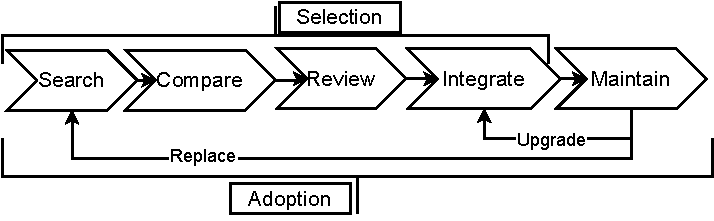
\includegraphics[scale=.7]{images/adoption-process.pdf}
    \caption{Software library adoption process}
    \label{fig:adoption-process}
\end{figure}
We found that developers go through five iterative steps of search, compare, review, integrate, and maintain for library adoption. \fig\ref{fig:adoption-process} shows how the five steps can support the selection and adoption process of software libraries. To the best of our knowledge, ours is the first study that presents an end-to-end adoption process like \fig\ref{fig:adoption-process} (explained further in \sec\ref{sec:phases}).

We reported seven organizational (e.g., lack of library adoption policy), individual (e.g., lack of experience), and industry-wide problems (lack of library selection tool) that hinder the library adoption process. To our knowledge, no prior study reported these barriers.

We found that developers follow six \principle\space (e.g., maximize flexibility during adoption) to achieve the optimum benefits from libraries and manage the burdens associated with those libraries. To the best of our knowledge, ours is the first study that reports and catalogs the \principle\space that define the developer behavior during the adoption of software libraries.

% \begin{itemize}[leftmargin=10pt]
% \item 

%     \item     
%     \item 
    
%     \item 
% \end{itemize}



\nd\bf{{RQ2. What tool supports are needed to guide developers during the adoption of third-party software libraries in an organization?}} Using the derived \model\space from RQ1, we conceptualized and evaluated a new library selection tool that can compare multiple libraries and generate a score for the better library based on the developers' priorities and conditions. We also explored whether large-language model-based chatbots can help developers in library selection. From the industry evaluation survey, we found that chatbots can only be used for initial information discovery but cannot be reliable for decision-making. In addition to our conceptual library selection tool, we offer seven recommendations that software companies and developers can follow to guide their library adoption process. 
%\begin{itemize}[leftmargin=10pt]
%    \item 
%    \item 
%\end{itemize}

In Table \ref{tab:contribution-summary} we outline the major contributions of our research and summarize how the contributions advance the literature in third-party software library selection and adoption.
% The outcome is a theoretical framework of software \model\space that consists of a catalog of processes, conditions, factors, sources, barriers, and {\principle} related to software library adoption in the industry. 
% % By conditions, we mean environmental characteristics which are independent of the library under consideration. Factors refer to the characteristics of the library itself. 
% In addition to deriving the model, we were also interested to conceptualize library selection tools to guide developers. With this objective, we formulated the following research questions:



% \nd\bf{RQ1: What is the library adoption model and its dimensions?}
% To explore this RQ, we further divided into six more sub-RQs.

% \nd\bf{RQ1.1: What behavior model developers follow while adopting libraries?} We derived a \model\space that can describe all the dimensions of library selection. The model is very similar to the business buyer behavior model in marketing theories \cite{kotler2014principles} while the adoption process is similar to consumer buying decision process. To our knowledge, this is the first time a library adoption model has been proposed that resembles well-established consumer marketing theories.

% \nd\bf{RQ1.2: What are the process developers follow in the industry during their adoption of a software library?}
% We found that developers go through five iterative steps of search, compare, review, integrate and maintain for library adoption. \fig\ref{fig:adoption-process} shows how the five steps can support the selection and adoption process of software libraries. To the best of our knowledge, ours is the first study that presents an end-to-end adoption process like \fig\ref{fig:adoption-process} (explained further in \sec\ref{sec:phases}).

% \nd\bf{RQ1.3: What are the major data sources developers use during their adoption decision of a software library?}
% During this process, software developers/teams collect library related information from five major information sources (e.g. online forums, colleagues, etc.). 



% \nd\bf{RQ1.4: What conditions influence the library adoption process?} We found that developers are influenced by 23 types of conditions (e.g., environmental, organizational, etc.) under 5 major categories (environmental, organizational, technological, team-specific, and individual).
% We identified 14 new conditions (e.g., geographic, criticality of feature) for the first time in our study in addition to 9 existing conditions reported in the literature.

% \nd\bf{RQ1.5: What library specific technical factors developers consider during the library adoption process?}
% We found that developers consider overall 28 types of factors (under four categories of technical, commercial, maintenance and external factors) during the library adoption process. 
% While 13 of these and factors are previously reported in the literature  (e.g., popularity), 15 others were observed the first time in our study (e.g., customer support, used by reputed organization).
% % As developers follow the adoption process and consider the influential conditions and factors, we found that their final decisions on whether and how to adopt a library can be encoded into several guiding principles. As such, we sought to answer the final research question as follows. 

% \nd\bf{RQ1.6: What challenges developers face while adopting software libraries} We reported 7 organizational (e.g., lack of library adoption policy), individual (e.g., lack of experience), and industry wide problems (lack of library selection tool) that hinders the library adoption process. To our knowledge, no prior study reported these challenges.

% \nd\textbf{RQ1.7: What \principle\space do developers follow during the library adoption process?} We found that developers follow 6 \principle\space (e.g., maximize flexibility during adoption) to achieve the optimum benefits from libraries and manage the burdens associated with those libraries. To the best of our knowledge, ours is the first study that reports and catalogs the \principle\space that define the developer behavior during the adoption of software libraries.

% After exploring RQ1, we were interested to apply the findings to guide developers in library selection process with the following research question:

% \nd\bf{RQ2: What tools do developers wish for to support their library selection?}

% Using the derived \model\space from RQ1, we conceptualized and evaluated a new library selection tool that can compare multiple libraries and generate a score for the better library based on the developers' priorities and conditions. We also explored whether large-language model-based chatbots can help developers in library selection. 
% From the industry evaluation survey, we found that chatbots can only be used for initial information discovery but cannot be reliable for decision-making.

% In addition to our conceptual library selection tool, we offer seven recommendations that software companies and developers can follow to guide their library adoption process. In Table \ref{tab:contribution-summary} we outline the major contributions of our research.








\section{Background and Related Work}
%\begin{table*}[]
    \centering
    \caption{Research works related with software, technology, and library selection and comparison tools and factors}
    \begin{tabular}{p{3cm}p{4cm}p{10cm}}
    \toprule
    \textbf{Output} & \textbf{Study} & \textbf{Summary} \\ 
    \midrule
    Software Evaluation Tool & Open source software evaluation factors and tool \cite{wasserman2017osspal,
    li2022exploring} & Provides evaluation criteria (factors) for open source software (not library component). Identified 8 factors and 74 sub-factors. \\ 
    Technology Comparison Tool & \textbf{DiffTech:} technology comparison tool \cite{huang2018tell, wang2020difftech, wang2021difftech} & The tool mines comparative opinions in Stack Overflow about pairs of technologies without any predefined selection factors. \\ 
    \textbf{Library factors} related data & \textbf{LibComp:} Quantitative data collection on library specific factors \cite{de2018library, de2018empirical, el2020libcomp} & Proposed 9 quantitative factors of libraries and developed an online tool and an IDE plugin to display library specific information. \\ 
    \textbf{Library factors} related opinion & \textbf{Opiner:} Opinion summarization of library specific factors \cite{uddin2017automatic, uddin2017opiner} & Developed an API opinion summarization tool by crawling online forums contents regarding posts related with different APIs and their aspects. \\ 
    Opinion Mining Technique & Opinion mining and sentiment analysis techniques \cite{lin2019pattern, uddin2019automatic, uddin2022empirical} & Prepared benchmark dataset for opinions, and proposed pattern based or machine learning based techniques. \\ 
    Library Related Needs & Developer needs identification from Stack Overflow \cite{liu2021api, uddin2019understanding} & Identified 8 API related needs expressed in Stack Overflow and reported library selection factors from developer survey. \\ 
    Library Comparison UI & User interface for library comparison \cite{yan2022concept} & The interactive user interface presents concept (aspect) annotated code examples side by side for comparing multiple libraries. \\ 
    \textbf{Library Factors} for selection criteria & Library selection factors \cite{spinellis2019select, larios2020selecting} & Presented library selection factors from experience and from practitioners' survey and interview. \\ 
    
    
    \bottomrule
    \end{tabular}
    \label{tab:related-works-summary}
\end{table*} % AB: Save this for the tool paper

In this section, we will first discuss the background of buyer behavior models which we used as the lens for viewing software library adoption. Next, we will consider two strands of literature which relate to our research questions. 



\subsection{Background}
\subsubsection{Buyer Behavior Models}
We use buyer behavior as the lens through which we examine software library adoption decisions.
In contrast to technology adoption models, consumer and business buyer behavior model drawn from marketing theories provide more in-depth insights into how a consumer or a business organization makes a decision to procure a product. In their seminal textbook, Kotler and Armstrong defined consumer/organization specific concerns as `influences' and  separated these from product-specific attributes (which we will henceforth refer to as factors, consistent with the software engineering literature) while explaining the influences in buying process \cite{kotler2014principles}. Moreover the product-specific factors are also a foundational element of the Fishbein Multiattribute Model which calculates the weighted average of all product-specific factors to define which product the consumer will select \cite{fishbein1967attitude}. Since it was introduced almost 60 years ago, this model has been ``extensively used by consumer researchers'' \cite{blackwell2001consumer}. %The segregation between product (here library) attributes and decision influences was established in marketing theory because of the elaborate analysis of the buying decision process. 
In addition to influential conditions, and important product factors, the buyer behavior models also provided steps of buying decision process and actors involved or influencing the product adoption. Though these models provide more holistic approach compared to technology adoption models, there is no study how such models are applicable to technology adoption specifically, library adoption process.

% By contrast, research on library selection has focused almost entirely on technological factors, and has not looked holistically at the entire library selection process while distinguishing product-specific factors from influences.
\subsection{Related Work}
 % In section~\ref{sec:tech-adoption}, we look at the steps of technology adoption, which relates to our first research question. Next, we approach our second and third research questions by discussing the factors used in evaluation and the formal processes which have been developed to facilitate the decision, usually at an organizational level. Section~\ref{sec:lit:automation} covers efforts that have been made to automate gathering information to facilitate software selection decisions.
\subsubsection{Steps of Technology Adoption} %% Background for RQ1
\label{sec:tech-adoption}
The process by which a tool comes to be adopted within an open source software community was found to consist of several phases: knowledge, individual persuasion, individual decision, individual implementation, organizational adaptation, and organizational acceptance \cite{krafft:2016:free}. In the knowledge phase, for example, sedimentation describes a technology gaining recognition to the point that it is considered ready for adoption. Marketing, or the active promotion of the tool or technique to generate excitement, simulates developers to evaluate the project's utility. The final knowledge phase, peercolation, explains how information spreads between peers and how this information from trusted sources leads to favored treatment of the technology.


% Considering all related works, there has been a vacuum and necessity for understanding the complete process and principles of library adoption (not only selection, rather than maintenance as well) and its process  which is performed in this study. 

In marketing, psychology, and technology literature, a number of technology adoption models have been proposed. Fishbein and Azjen's Theory of Reasoned Action (TRA) \cite{flanders1975belief-tra} explaining consumer's belief, attitude, intention, and behavior has become foundational base for investigating personal technology usage \cite{taherdoost2018-adoption-models}. Two notable derivation of TRA model are Theory of Planned Behavior (TPB) \cite{ajzen1991-tpb} which added perceived behavioral control and Technology Acceptance Model (TAM) \cite{davis1985tam, davis1989-tam-usefulness} which considered perceived usefulness, perceived ease of use, and attitude toward use for technology adoption by individual consumers. While these models explained consumer behavior to adopt or accept a technology product, TOE Framework by Tornatzky et al. \cite{tornatzky1990processes-toe} describes how the adopting and implementing technology in organizations is influenced by Technological, Organizational, and Environmental (TOE) conditions. Whereas TOE framework provides insights how organizational adoptions could be influenced, this framework has been criticized to be too generic \cite{zhu2005post-toe-critic} and not sufficient enough for explaining software library adoption process.



\subsubsection{Technology Selection Factors and Processes}\label{sec:lit:processes}

Perhaps the most obvious factors involved in the selection of libraries relate the the needs of developers and the utility offered by the library. Historic factors which limited software reuse were limitations in the capacity of retrieval technologies to return relevant results \cite{hummel2008code}. Retrieval is no longer a serious concern, as modern software ecosystems have developed that make it easy for developers to incorporate libraries with searches built in to IDEs. However, the evaluation of components remains difficult, especially when the process can be hidden to the extent that malicious code can be hidden in dependency chains of popular packages \cite{wyss2022wolf}. Developers seek out API reviews in order to discover information related to their specific development needs and to compensate for shortcomings in the official documentation \cite{uddin2019understanding}. Liu et al. created a taxonomy of the API elements required by developers based on an analysis of Stack Overflow posts, identifying categories such as non-functional improvement, error handling, and API usage learning \cite{liu2021api}. Developers make use of a ``combination of code examples and opinions about an API as a form of documentation,'' relying on the positive and negative views in order to assess the quality of the API \cite{uddin2019understanding}. This is complicated by concerns about the trustworthiness, relevance, and recency of the opinions. % Also uddin2019understanding

While the aforementioned studies have focused largely on technical aspects of library selection, Larios-Vargas et al. conducted the most comprehensive study of factors associated with library selection, identifying 26 through semi-structured interviews, which were subsequently validated through a survey of 116 developers \cite{larios2020selecting}. The factors were categorized as technical, human, and economic. In contrast to our study, they did not investigate the conditions under which each factor is relevant in the selection process. Furthermore, the study did not draw a clear distinction between factors that are directly related to the libraries, and those which stem from the external environment, such as company culture, company management, and type of industry. These concerns undoubtedly influence the selection process, but the lack of segregation of library-specific factors and conditions, together with the lack of guidance on the when factors should be considered limits the extent to which the study can support the decision-making process.

% Shorter version of paragraph.
Companies trying to select the most appropriate library for a task have been provided with processes - sometimes with tool support - which strive to help them compare factors based on their internal conditions, such as Qualification and Selection Open Source (QSOS) and Open Business Readiness Rating (OpenBRR) \cite{deprez2008comparing, semeteys2008method, wasserman2017osspal}. Li et al. also identified eight key evaluation factors in considering OSS applications (e.g., community and adoption, development process, etc.) \cite{li2022exploring}.  Cruz, Wieland and Ziegler proposed a process which considers the scenario for adopting, the requirements, the interpretation of collected information, and an investigation of the criteria \cite{cruz2006evaluation}. For each scenario, the authors identify the functional, technical, organisational, economical, and political requirements associated with it. While these attempts to codify the decision process do address human and technical factors, they are primarily focused on the selection of applications and tools, not libraries.
%% Long version of paragraph below.
% There have been multiple processes proposed for companies trying to select the most appropriate open source software for a task. Although the emphasis is typically on products, libraries are occasionally mentioned and indeed, there is nothing in the processes which would rule out their use on components. Two such processes, both of which are based on a comparison of factors based on conditions, are Qualification and Selection Open Source (QSOS) and Open Business Readiness Rating (OpenBRR). \cite{deprez2008comparing}. In QSOS, the user begins with a list of projects which seem to fit the overall requirements, evaluates them according to the criteria given by QSOS (such as intrinsic durability, technical adaptability, and documentation), adjusts the importance of each criterion based on their conditions, and then makes a decision \cite{semeteys2008method,deprez2008comparing}. OpenBRR reduces a long list of projects to a short list of candidates based on the criticality of the system and context-specific criteria such as age of the project and quality of source code. OpenBRR proposes eight key considerations: licensing, standard compliance, referencable adopters, availability of support, implementation language(s), third-party reviews, books, and review by industry analysts; a tool was developed to help developers follow the process \cite{deprez2008comparing,wasserman2017osspal}. Li et al. also identify eight key evaluation factors in considering open source software applications: community and adoption, development process, economic, functionality, license, operational software characteristics, quality, and support and service \cite{li2022exploring}. Cruz, Wieland and Ziegler proposed a process which considers the scenario for adopting (the user's situation), the requirements, the interpretation of collected information, and an investigation of the criteria \cite{cruz2006evaluation}. For each scenario, the authors identify the functional, technical, organisational, economical, and political requirements associated with it; for instance, when using open source software to reduce costs, economic considerations include sustainability, protection of investment, cost reduction, and division of development costs.

There have been numerous attempts to provide automatic support for technology evaluation. In a study of industry requirements for governance of OSS libraries, Harutyunyan, Bauer and Riehle identified that such a tool should aid in searching for libraries, selecting the best library, and estimating the cost of using the library \cite{harutyunyan:2018:understanding}. Existing tools, such as DiffTech, LibComp, Opiner, and POME, have focused on these first two requirements \cite{huang2018tell, wang2020difftech, wang2021difftech,de2018library, de2018empirical, el2020libcomp,uddin2019automatic, uddin2022empirical,lin2019pattern}. 
These tools rely on a variety of data sources. Another approach involved displaying annotated code examples \cite{yan2022concept}. What these tools have in common is that they each focus on a subset of aspects involved in the decision, and are unable to consider developer's specific priorities.

% Library selection
%\subsubsection{Automation of Technology Evaluation}\label{sec:lit:automation}

%As the majority of programmers make use of tools such as search engines, code-specific search engines, and other resources in their selection of libraries \cite{umarji2008archetypal}, it is unsurprising that there have been several attempts to aid developer selection by developing tools to automate the comparison of libraries. In a study of industry requirements for governance of open source software libraries, Harutyunyan, Bauer and Riehle identified that such a tool should aid in searching for libraries, selecting the best library, and estimating the cost of using the library \cite{harutyunyan:2018:understanding}. Existing tools have focused largely on the first two requirements. DiffTech presents a side-by-side comparison of 2,410 pairs of technologies based on mining and clustering opinions from Stack Overflow \cite{huang2018tell, wang2020difftech, wang2021difftech}. The results highlight the factors that developers consider important in the comparison of two alternatives, but the approach is specific to the technologies studied and cannot be generalized to provide advice on decisions about other technologies. LibComp uses nine metrics to suggest Java libraries to developers through an IDE plugin \cite{de2018library, de2018empirical, el2020libcomp}. These metrics are automatically derived from the library repository and include measures such as popularity, release frequency, and issue response time. These may help developers answer questions about the sustainability of the software, one of the factors Spinellis advised examining in an experience paper on open source software selection \cite{spinellis2019select}, but it does not address other possible considerations, such as the appropriateness of the technology to the task. One attempt at addressing this problem involved displaying annotated code examples of user interfaces presented side by side \cite{yan2022concept}. Opiner is similar to LibComp in that it provides users with rankings based on factors, but the factors were determined through a study of users \cite{uddin2019automatic, uddin2022empirical}. Opinion mining and sentiment analysis techniques are used to create the evaluation. Meanwhile, Lin et al. also proposed pattern based mining technique `POME' with superior performance \cite{lin2019pattern}.   

%Moving from factors primarily of interest to developers to evaluation processes aimed at organizations, Wasserman et al. developed a tool to automate part of the OpenBRR process by collecting quantitative data from a source code repository, and qualitative reviews submitted to an online portal \cite{wasserman2017osspal}. Of the 74 sub-factors Li et al. identified as related to the evaluation of open source software applications, based on 170 metrics, 40 sub-factors can be regularly obtained through source code repositories, leading the authors to conclude that information provided about projects is often insufficient for consideration \cite{li2022exploring}.

\subsubsection{Technology Specific Library Selection} Several library specific studies have been conducted focusing on specific technology or scenarios. For example, there are library recommendation techniques for Android technology \cite{moataz2020android-reco} and for library migration scenarios \cite{he2021migration}. Since Android operating system evolves faster, library upgrade is an important issue and few studies attempted to analyze the upgrade scenarios and found that 98\% libraries with security vulnerabilities are not updated, 28\% of Android applications lag in average 16 months behind latest library version \cite{aerr2017android-update, mcDonnell2013android-update-lagging, polese2022android-integration-history}. Few research have been conducted to identify the characteristics of popular library in different programming languages such as Java, Android, and JavaScript and found that popular libraries are more well-documented and can be more unstable \cite{sujahid2023popular-javascript, lima2020popular-characteristics}. A study on data science libraries revealed that developers in data science and general software engineering have different priority of library specific factors \cite{nadi2023datascience}. Literature review on software library or package selection studies has remarked that there is a need to develop a framework for software evaluation and selection  methodology \cite{jadhav2009review}.


\section{Methodology}\label{sec:methodology}
Given the absence of a library adoption model in the literature, we decided to adopt Straussian grounded theory \cite{corbin2014gt} to derive such a model.  
% All of the authors of this paper have at least ten years of industry experience. As such, it was also important that our formulation of the library adoption model is derived from the responses of study participants, while the model is not biased by our prior own experience. 
% Unlike classical grounded theory, Straussian grounded theory acknowledges the presence of research bias, assumptions, and motivations, and provides structured tools (constant comparison and memoing) to handle the intrusion \cite{stol2016grounded,corbin2014gt}. 
We chose to conduct semi-structured interviews of industry developers to learn about the model because such interviews allow us to elicit unexpected information and to evolve our questions as the study progresses \cite{HoveAnda, Seaman}. 
Figure~\ref{fig:methodology} provides an overview of the overall research method which was applied to the study.
\begin{figure*}
    \centering
    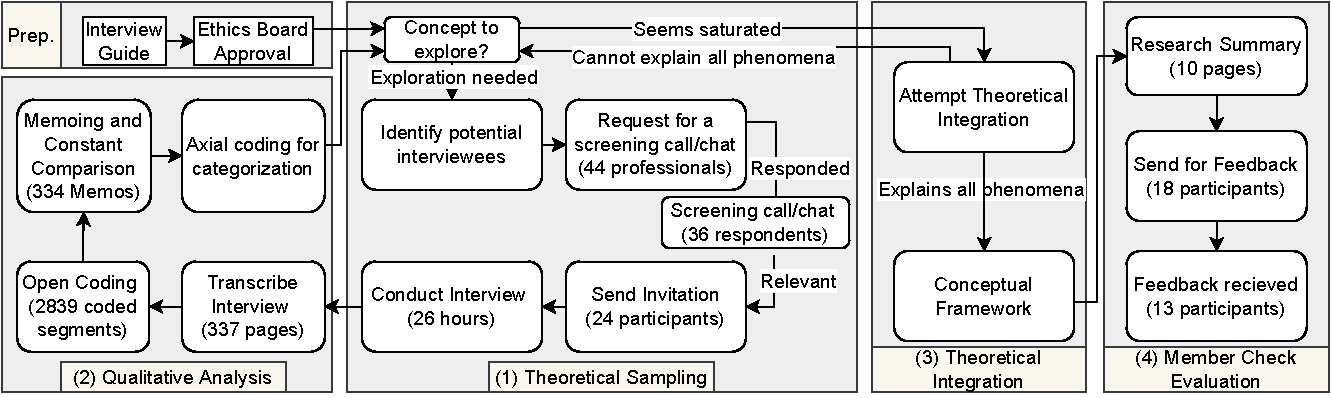
\includegraphics[scale=.7]{images/methodology.pdf}
    \caption{Grounded theory research method applied}
    \label{fig:methodology}
\end{figure*}



% Because the study involved human subjects, we obtained approval from the Ethical Review Board of our institution before conducting interviews. In total, we conducted \numInterviews interviews, interleaving data collection and analysis following grounded theory design principles. Figure~1 in the Appendix shows the overall research process.




% \begin{table*}[]
%     \centering
%     \begin{tabular}{p{.4cm}r{.4cm}l{2.5cm}l{2cm}l{2cm}l{2.2cm}r{2cm}r{1.5cm}}%{lrllllrr}
% \toprule
% P\# & Yrs & Role & Primary Tech & Continent & Industry & Company Size & Tech Size \\
%     \midrule
% P1 & 12 & Architect & Java & Europe & Automotive & 4000 & 500 &  \\ 
% P2 & 6 & Software Engineer & Python & North America & Cloud Service & 150000 & 80000 &  \\ 
% P3 & 12 & Software Engineer & Android+iOS & North America & Automotive & 30000 & 600 &  \\ 
% P4 & 20 & CEO & .NET, AWS & Asia & Broadcast Media & 60 & 54 &  \\ 
% P5 & 16 & Engr. Manager & .NET, AWS & Australia & Financial & 40 & 12 &  \\ 
% P6 & 17 & Software Engineer & Perl & Europe & Tech & 200 & 20 &  \\ 
% P7 & 9 & CTO & Javascript & North America & Data Analytics & 21 & 6 &  \\ 
% P8 & 9 & Software Engineer & Any Tech & North America & Cloud Service & 20000 & 10000 &  \\ 
% P9 & 13 & Architect & Python & North America & Web & 250 & 100 &  \\ 
% P10 & 15 & Software Engineer & Javascript & Europe & Energy & 11000 & 300 &  \\ 
% P11 & 7 & ML Engineer & Python & North America & Data Analytics & 100 & 30 &  \\ 
% P12 & 22 & Consultant & Perl & Asia & Tech & 30000 & 1000 &  \\ 
% P13 & 15 & Architect & Java & North America & Retail & 1000000 & 200000 &  \\ 
% P14 & 6 & Software Engineer & Android+iOS & Asia & Financial & 150 & 100 &  \\ 
% P15 & 22 & CTO & .Net & Asia & Enterprise & 350 & 300 &  \\ 
% P16 & 9 & Software Engineer & Java & Asia & Cyber Security & 400 & 300 &  \\ 
% P17 & 15 & CTO & Ruby on Rails & Europe & Custom Software & 35 & 6 &  \\ 
% P18 & 27 & CEO & C++ & North America & Financial & 150 & 40 &  \\ 
% P19 & 15 & Engr. Manager & Ruby on Rails & North America & Cloud Service & 150000 & 75000 &  \\ 
% P20 & 10 & Software Engineer & Android+iOS & North America & Food Service & 70 & 10 &  \\ 
% P21 & 13 & Software Engineer & Ruby on Rails & North America & CI/CD & 1800 & 900 &  \\ 
% P22 & 30 & Architect & Java & North America & Operating Sys. & 19000 & 9000 &  \\ 
% P23 & 7 & ML Engineer & Python & South America & Custom Software & 900 & 750 &  \\ 
% P24 & 6 & ML Engineer & Python & North America & Medical & 150 & 80 &  \\ 

%     \bottomrule
%     \end{tabular}
%     \caption{Interview participant's Professional profile along with the industry and size of their companies}
%     \label{tab:participants}
% \end{table*}


\begin{table}[]
    \centering
    \begin{tabular}{p{.4cm}p{.4cm}p{.5cm}p{.8cm}p{.5cm}p{2.2cm}r{.5cm}}%{lrllllr}
\toprule
P\# & Yrs & Role & Tech & GEO & Industry & Tech Size \\
\midrule
P01 & 12 & Arc & JV & EU & Automotive & 500 &  \\ 
P02 & 6 & SDE & PY & NA & Cloud Service & 80,000 &  \\ 
P03 & 12 & SDE & A/IOS & NA & Automotive & 600 &  \\ 
P04 & 20 & CEO & .NET & AS & Broadcast Media & 54 &  \\ 
P05 & 16 & EM & .NET & AU & Financial & 12 &  \\ 
P06 & 17 & SDE & PE & EU & Tech & 20 &  \\ 
P07 & 9 & CTO & JS & NA & Data Analytics & 6 &  \\ 
P08 & 9 & EM & Any & NA & Cloud Service & 10,000 &  \\ 
P09 & 13 & Arc & PY & NA & Web & 100 &  \\ 
P10 & 15 & EM & JS & EU & Energy & 300 &  \\ 
P11 & 7 & MLE & PY & NA & Data Analytics & 30 &  \\ 
P12 & 22 & Cons & PE & AS & Tech & 1,000 &  \\ 
P13 & 15 & Arc & JV & NA & Retail & 200,000 &  \\ 
P14 & 6 & SDE & A/IOS & AS & Financial & 100 &  \\ 
P15 & 22 & CTO & .NET & AS & Enterprise & 300 &  \\ 
P16 & 9 & SDE & JV & AS & Cyber Security & 300 &  \\ 
P17 & 15 & CTO & RoR & EU & Custom Software & 6 &  \\ 
P18 & 27 & CEO & C++ & NA & Financial & 40 &  \\ 
P19 & 15 & EM & RoR & NA & Cloud Service & 75,000 &  \\ 
P20 & 10 & SDE & A/IOS & NA & Food Service & 10 &  \\ 
P21 & 13 & SDE & RoR & NA & CI/CD & 900 &  \\ 
P22 & 30 & Arc & JV & NA & Operating Sys. & 9,000 &  \\ 
P23 & 7 & MLE & PY & SA & Custom Software & 750 &  \\ 
P24 & 6 & MLE & PY & NA & Medical & 80 &  \\ 

    \bottomrule
    \end{tabular}
    \caption{Interview participants by years in industry, role (Arc-Architect, EM-Engineering Manager, Cons-Consultant, SDE-Software Development Engineer, MLE-Machine Learning Engineer, CTO-Chief Technology Officer), primary technology (JV-Java, PY-Python, A/IOS-Android/iOS, PE-Perl, JS-JavaScript, RoR-Ruby on Rails, Any-not limited by technology) geographic location (AS-Asia, AU-Australia, EU-Europe, NA-North America, SA-South America), industry, and company tech size.}
    \label{tab:interviewee-profile}
\end{table}

\subsection{Participant Recruitment Strategy}
We conducted \numInterviews interviews between June 2022 and January 2023. Table~\ref{tab:interviewee-profile} provides an overview of participants.
The average number of years of professional experience of the participants was 14 years. Their roles spread across the spectrum of engineering and leadership roles and in nine different countries from five continents. The tech stack also had wide varieties (e.g., C/C++, Java, Python, Android, iOS, .NET, machine learning, etc.). Many of our participants were working in large corporations (e.g., Google, Microsoft, etc.) and open-source projects. Among all the interviewees, three experts identified themselves as female. Our participants covered 16 application domains including specialized regulated areas as such health, finance, cybersecurity, and broadcast media. 

 % An important part of grounded theory is theoretical sampling of the concepts. It means that after every interview, we had to perform data analysis of the interview, identify the concepts which needed further elaboration, and select the next few interviewees to improve the probability of getting answers regarding emerging concepts. Before conducting interviews, we performed initial screening of the participants through a short phone call (around 5 to 10 minutes). After we identified that a participant could provide relevant insights, we sent them a formal interview invitation. 
 % In this way, we reached out to 38 potential participants for initial screening of emerging concepts through the professional network of the authors. 



\subsubsection{Theoretical Sampling for Recruitment}
\begin{table*}[]
    \centering
    \begin{tabular}{p{.4cm}p{4cm}p{6cm}p{6cm}}%{llll}
    \toprule
    P\# & Concept we wanted to enhance & Why we selected this Participant & Concepts they enriched significantly \\ 
    \midrule
P1 & Initial process and factors & Architect of a large system & Library definition, factors, influences \\ 
P2 & Licensing and Security Issues & Working in a large structured company & License, company technology \\ 
P3 & Mobile development Factors & 12+ years experienced in mobile application & Cost, company tech, comparison  \\ 
P4 & Long term maintenance concerns & Being a CEO, takes decisions considering long term impact & Company application domain, active development of library \\ 
P5 & Decision making processes & Stablishing the processes in a startup team & Information search, company culture \\ 
P6 & Open Source factors & Has experience regarding OSS contribution and research & Open source, Personal motivation \\ 
P7 & Factors for a startup & Being a startup CTO may share different priorities & Flexibility, Ease of Installation, Community Support \\ 
P8 & Performance factors & Working in a cloud company that may requiew high performing libraries & Familiarity, Team Discussion, Library Migration \\ 
P9 & Migration scenarios & Experienced to migrate company tech stack as architect & Legal risks, Lack of Stability, Less prefered than native support \\ 
P10 & Visualization and front end libraries & Working as web developer for over a decade & Customer support, flexibility, existing repository \\ 
P11 & Machine learning libraries & Experienced in machine learning in gradudate research studies and in industry & Talk to people, Performance, Outstanding library selection \\ 
P12* & DevOps Process for Library Security Issues & Consulted dozens of companies in DevOps process establishment & Barriers of library usage, Baggage of libraries \\ 
P13 & Selection process in large organizations for legal and security risks & Has been an architect in a large team for 10+ years & Consent Process, Benefits of libraries, Tech Expert Opinion \\ 
P14 & Library migration scenarios & Experienced in managing mobile apps with large user base in all platforms & Make life easy, Life long maintenance, Migration to other library \\ 
P15 & Organizational process and motivation for libraries & Experienced in organization process since increased dev team from 3 to 300 & Delivery Deadline, Don't Reinvent the wheel, Feature criticality \\ 
P16* & Process of security concerns & Cerified security professional actively developing security products & License issues, Data Transfer Security, Geographic Impact  \\ 
P17 & Security Process & Delivers custom software to customers and maintains SecOps in CI/CD & Post Integration Maintenance for Security \\ 
P18 & C++ libraries in large scale long term products & Leads development of a 30 year old product written in C++ with 2M lines of code & Lifelong Maintenance Burden, Compatibility, Uniform Coding Style \\ 
P19 & Company Culture, Open Source, Concept Saturation & Experienced working in start-up and large organizations who open source libraries & Standard practices in large organizations, Considerations in open source \\ 
P20 & Challenges in mobile application libraries, Concept Saturation & Full career in mobile app development, mostly in iOS which requires more maintenance & Lifelong Maintenance Burden, Abandoned Libraries, Migration \\ 
P21 & Company Culture, Open Source, Concept Saturation & Works full-time in a prominent open core company & Company policies, Guiding Principles \\ 
P22 & Guiding Principles, Open Source & Experienced in persuing large corporation for open source library adoption & Guiding Principles \\ 
P23 & ML libraries & Working in South America in ML domain & ML Library Dependency Issues \\ 
P24 & Company Culture, Industry, ML Libraries & Working in health sector using ML libraries extensively. & ML Library deployment and upgrade issues \\ 

\bottomrule
    \end{tabular}
    \caption{How we recruited interview participants following theoretical sampling for Concept Saturation. (We could not enhance targeted concepts from the *-marked participants (P12, P16), rather enriched other important concepts.)}
    \label{tab:theoritcal-sampling}
\end{table*}
We started with an architect (participant P1) from our professional acquaintance who had twelve years of experience including designing and developing from scratch a payment system in a 260 human-year project spanning over six years. We knew that they had to select a huge number of libraries throughout this development. Our first interview lasted  115 minutes, as we were developing initial concepts around all of our research questions, while subsequent interviews averaged 64 minutes. % range 42-115
After analyzing the initial interview data, we realized that we needed more information about commercial factors (particularly licensing) and the integration process of a library. Hence, we chose our next participant (P2) who was working in a large organization (\#engineers $\geq$ 80K), and who had experience with licensing concerns about software libraries. In this way, we continued the theoretical sampling to saturate all the relevant concepts. We recruited the interviewees from the direct or extended professional networks of the three authors each of which had more than ten years of software industry experience. Before any interview, we conducted a screening call or email conversation to confirm the relevance of the interviewee regarding the specific concept we wanted to explore. The motivation for selecting every participant is provided in the table \ref{tab:theoritcal-sampling}. 
% In most of the cases, we were able to extract insights about target concept from the interviewees. For example, we wanted to dig deep into the library maintenance issues and we identified mobile applications need continuous update because of the yearly operating system update. Hence we reached out to a mobile developer P14 who actively manages applications in all mobile OS platforms and in the interview, they provided us significant insights about maintenance and migration issues. 


\subsubsection{Concept Saturation over the Interviews}
\begin{figure*}
    \centering
    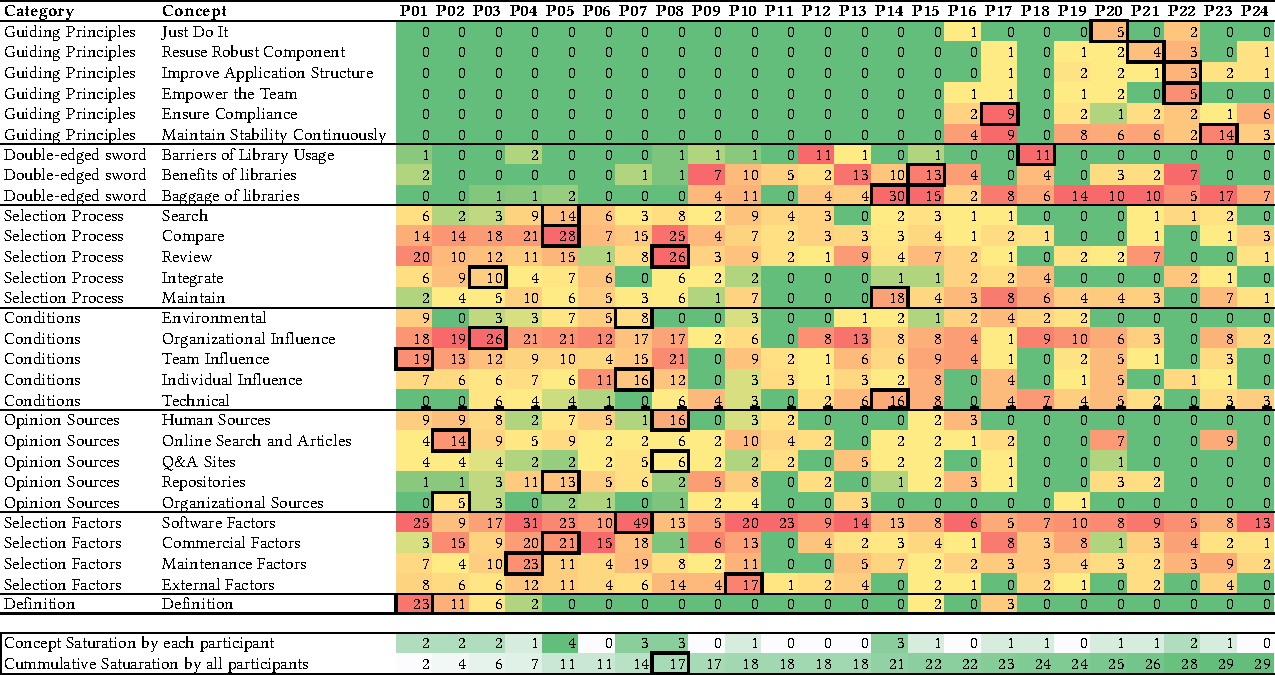
\includegraphics[scale=0.8]{images/saturation.pdf}
    \caption{Heatmap of concept saturation over the interviews. Red refers to higher discussion of a concept by an interviewee, the number refers to how many times interviewee has discussed a concept. Green refers to lower discussion of concepts by an interviewee.}
    \label{fig:saturation}
\end{figure*}
Figure~\ref{fig:saturation} shows how the concepts were discussed during each interview. The number denotes how many times a concept was discussed by one particular interviewee. The more a participant discussed a particular concept, the more red the corresponding cell is. For example, the library search concept was most discussed by P5 (14 times). After their interview, subsequently, we did not have much to discuss the search process, for example, P10 also discussed the same concept 9 times. Hence after we reach a maximum number of times a concept has been discussed, we consider that the concept is saturated. Still, for the sake of a uniform discussion with the interviewees, we keep discussing the concepts in case any new corner case comes up. Whereas library selection factors were saturated by P10 (external factors concept were most discussed by P10 and then gradually declined in consecutive interviews), the conditions and the selection process were saturated by the interview of P14. However, it took us interviews till P18 to attain maximum discussion of barriers to library usage (11 times) and P23 to saturate the concept of maintaining continuous stability. By the time we interviewed P24, no further concepts were discussed and all previous concepts were saturated well beforehand. 

% Our work was initiated with the question RQ1: ``What are the major steps developers follow during their adoption of a software library?'' We soon realized that the process is influenced by certain conditions and factors, leading us to ask RQ2: ``What conditions and technical factors influence the library adoption process?'' 
% %As we continued to conduct interviews, our concepts started to saturate. Though many interviewees contributed towards the saturation, a few interviewees contribute most, and after such an interview a concept saturates very quickly. 
% By time we interviewed P8, we also realized that there were specific library selection principles and many pros and cons of libraries depending on the scenarios. Also after hearing P9's concerns about third-party libraries, we started to discuss about benefits and barriers more. This led to RQ3: ``What guiding principles do developers follow in library adoption?'' These concepts were well understood by the time we interviewed P22. The concepts and principles all saturated by the time we completed our last interview (i.e., P24).

%\textcolor{blue}{[Minaoar]}
%Our work was initiated by the following question: \textit{\textbf{RQ1:} How developers adopt third-party libraries?} After understanding the adoption process, we realized that the process is influenced by certain conditions and technical factors. Then we tried to answer \textit{\textbf{RQ2}: What conditions and technical factors influence the library adoption process?} Finally, we were curious why developers change adoption process based on the conditions and factors? Is there any guiding principles developers follow for library adoption? Then our final question was \textit{\textbf{RQ3:} What guiding principles developers follow in library adoption?} \ab{I'd put this in the methodology where you're talking about GT}

% \subsubsection{Repeated Interviews for Open Questions}
% However, in few cases, we could not find elaboration of our target concept from the interviewee and had to plan for other participants who could answer the questions we had. For example, we expected that P12, who specializes in DevOps process establishment in tech companies, could share experience on continuous monitoring of libraries for security concerns. However, P12 explained that in most of the cases when they consulted the organizations, they could never reach up to that matured security monitoring level, their target was to achieve continuous functional test coverage up to 50\%. Though we could not elicit the target concept, we could collect valuable insights about the reservations organizations have towards open source libraries. Then we interviewed P16, who was a certified security professional actively developing security products, to know their security protection against software libraries. They again did not follow any continuous monitoring process, they only ran security audits once a year. Finally, we got a clear conception on continuous security monitoring for third-party libraries from P17. 

% \subsubsection{Profile of the Interviewees}
% Following the theoretical sampling, we stopped the interviews when we had properties and dimensions of all concepts. The average number years of professional experience of the participants was 14 years, and their roles spread across the spectrum of engineering and leadership roles, including engineer, architect, consultant, CTO and CEO who are working in nine different countries on five continents. The tech stack also had wide varieties, e.g., open source library intensive languages such as Java, Python, Perl, JavaScript, Android, and iOS, and also historically less library focused languages such as C/C++ and .NET. Many of our participants have professional experience of working in large corporations such as Microsoft, Google, Amazon, AWS, Oracle, Cisco, IBM, and open source projects such as GitLab, RedHat Enterprise Linux, and Azure Communications Services, as well as leading startup and small size companies with 6 to 10 developers. Three of the participants described more than 90\% of their full time work in open source projects. Among all the interviewees, three experts identified themselves as female. Our participants also covered a wide range of 16 application domains including specialized regulated areas as such health, finance, cybersecurity, and broadcast media. 

% \subsubsection{Interviews}
% We conducted \numInterviews interviews between June 2022 and January 2023. All interviews were conducted online using Microsoft Teams for easy transcription. All interviews were both audio and video recorded except one. Interviews lasted from 42 minutes to 115 minutes with an average of 64 minutes per interview. Because of lack of accuracy of auto-transcription, each interview was manually corrected. % In average, it would take around 12 hours to conduct and analyze each interview (interview process 2 hours, transcription 4 hours, coding 4 hours, memoing 2 hours) amounting to around \td{288} hours of manual work.

\subsection{Interview Data Collection and Analysis}
All interviews were conducted online using Microsoft Teams for easy transcription. All interviews were both audio and video recorded except one. 
%Interviews lasted from 42 minutes to 115 minutes with an average of 64 minutes per interview. 
Because of the lack of accuracy of auto-transcription, each interview was manually corrected.  
Qualitative data analysis (QDA) was interwoven with interviews. We used the qualitative data analysis tool MaxQDA
\cite{website:maxqda} for coding, memoing, and diagramming. The coding process consisted of open coding, axial coding, and theoretical integration. 
% Coding and categorization was done through the hierarchical Code System feature, while interview segments were annotated with In-Document Memos. The Code Matrix Browser was used to track emerging concepts. We used the In-Document Memo feature to sort memos and compare and refine the concepts to generate central categories. MaxMaps was used to create a hierarchy of codes and the process flow of library selection.

\subsubsection{Open Coding and Memoing} During each interview, we continuously took field notes so that we could identify our concerning points. After each interview, we made summary memos with the new concepts that emerged, the properties of existing concepts that saturated, and the questions that arose. After the first couple of interviews, the concepts had been identified and we were able to begin open coding after each interview. Initially, all codes were categorized under either of the process, factors, sources, and conditions concepts. As the number of interviews increased, major concepts of decision patterns and barriers emerged and we also increased memoing for concepts and questions which were emerging. The memos contained our thoughts regarding the opinions shared by the interviews. We were also constantly comparing opinions provided by a new participant with previously analyzed data. 

\subsubsection{Axial Coding} After coding and analyzing the first four interviews, we started to discover the intersection points of different concepts using axial coding. For example, we identified that some selection factors are related to technical issues such as \code{ease of use}, \code{performance}, and \code{compatibility}, whereas a few factors are not dependent on the software of the library itself, such as \code{active development}, \code{community support}, \code{paid customer support}, which mostly relate with central concept of \code{support and maintenance}. Similarly, \code{company culture} and \code{company technology} had a central theme of \code{organizational influence}, which differs from developer's \code{personal background}, \code{experience level} or \code{personal motivation} which fall under the \code{individual influence} category. Using axial coding analysis, we created another layer of categories to group similar factors, conditions, sources, processes, barriers, and decision principles. 

% \subsubsection{Memoing} As the number of interviews increased, we also increased memoing for concepts and questions which were emerging. The memos contained our thoughts regarding the opinions shared by the interviews. We were also constantly comparing opinions provided by a new participant with previously analyzed data. Sometimes if there is any contradiction among interviewees, we wrote memos how the experts were contradicting and what were the underlying reason they expressed different opinions. For example, P10 (a web developer) and P14 (mobile app developer) shared differing experience regarding library version upgrades, and we noted this memo: \textit{"According to P10's experience, if a major library upgrades its version, then other dependent libraries also keep track of the upgradation and keep their (dependent) libraries updated as well. However, from P14's experience of mobile OS upgradation, they faced deprecated libraries which were no longer supported. Why they are experiencing opposite situations? Is it because mobile operating systems upgrade more frequently than backend infrastructure and mobile library developers cannot keep up with the changes and leave the projects?"}

\subsubsection{Theoretical Integration} 
% The version of Straussian grounded theory we employed, published in 2014, differed from the earlier version by placing emphasis on theoretical integration rather than selective coding to generate the core concept \cite{strauss1998basics,corbin2014gt}.
Diagrams and memos helped us conduct theoretical integration to generate the core concept of our research. For example, we started the interviews and analysis to explore how the developers adopt libraries. As the analysis progressed, we attempted to generate a core concept by sorting the memos and drawing interactive diagrams. We realized that unless we deeply understood why developers use libraries, we could not generate a core concept. After we identified developers' motivations and concerns for third-party libraries, the core concept emerged as the decision patterns of software library adoption which in an organization can guide a developer to make a decision by employing the library adoption steps and by considering the factors and conditions that influence the steps. 
%\gias{give a concrete example of how a guiding principle is derived using theoretical integration} 
For example, few developers wanted to talk to people when they were under tight deadlines \emph{``the way of choosing libraries was actually talking to peers because we were in a rush to deploy" (P16)}. So we thought \code{Meet deadline} was a core concept. However, we also found that even when there was no deadline, some developers still reached out to their peers, because they did not want to spend time searching the library: \emph{``They [friends or colleagues] already did it, right? They can just tell you do this." (P11)} %{P11}
They wanted to \code{make their life easy}. Connecting these two motivations, we came to the conclusion that both of them followed a common decision pattern of \code{Just Do It}. 
% but in completely different conditions. In this way we could explain all types of developer decisions by following the guiding principles and these became the core concept of our library adoption model.

% , which was related with other concepts of the library factors, selection process, and conditional influence on the adoption.

% When we were asking why developers use libraries, suddenly an interviewee (P12) responded, \textbf{'Let me tell you why developers DO NOT use libraries'}. That was a ureka moment for us that led to the core concept of double-edged sword, and explained why developers consider so many factors and their complex organizational and technical conditions. Later using the sorted memos and interactive diagrams, we performed the theoretical integration to generate the theoretical framework of library adoption based on the core concept of a double-edged sword - \textbf{'win the battle with a double-edged sword, be careful lest it cuts you back'} or 'make your life easy, use a library instead, just be careful of the baggage it brings in.'

%\subsection{Data Availability}
%We include the following documents in our supplementary material: \todo{add reference to supplementary material - final version on zenodo \cite{website:replication-package}}
%\begin{itemize}
%\item Interview script
%\item Invitation emails containing adjusted interview script
%\item Consent form
%\item REB approval
%\item Final codebook exported from MaxQDA in Excel and MaxQDA format
%\item Grounded theory evaluation results of the study
%\item Appendix
%\end{itemize}
%In order to preserve the anonymity of our participants and to adhere to our ethics approval, we do not share a list of interview participants or the interview transcripts.


\section{Results}
\subsection{Library Adoption Life Cycle (RQ1)}\label{sec:rq1}
\subsubsection{Conceptual Framework}\label{sec:framework}

After the interleaved data analysis and interviews, we discovered two things that we did not assume at the beginning of the study. First, library adoption is not a one-off selection event, rather it has a complete life cycle involving selection, integration, and post-integration maintenance. Secondly, in addition to all the benefits libraries offer, they also have disadvantages, such as legal risks with licenses and life-long upgrades of library versions. The benefits are seen in the following quote:
\qi{I have used many third party libraries because they are ready to use tools, right? If I don't use them, I need to spend lots of time to develop my own libraries to do like sometimes very simple stuff. I think like it seems simple but when you get to the bottom of it, it will take time to do some let's say preprocessing or processing on the data that you have. But by using the third party libraries you can just import it and use the functions and it's very easy to use and very fast and user friendly.}{P11}

Evidence of disadvantage is illustrated by the following quote:
 \qi{There can be flaw within the library that could introduce security flaw and attacks to your system. It is always, always risky when you build a core component on top of a library and the library is not getting developed.}{P15} 
 
We found that under complex organizational context, developers tend to follow certain guiding principles (knowingly or unknowingly) to extract the right benefits and to tackle the disadvantages of the libraries throughout the whole adoption process. Hence, guiding principles became the central theme of the library adoption life cycle. The other aspects of the library adoption life cycle are conditions, factors, and information sources. The relationship between these different aspects is shown in Figure~\ref{fig:framework}, while the aspects are introduced below.

The lifecycle has five major steps, during which factors are considered and information is sought. The steps are:
\begin{inparaenum}[(P1)] 
\item information search, 
\item comparison of short-listed libraries, 
\item review of decision, 
\item integration into application, and finally 
\item life long maintenance.
\end{inparaenum} 
These are discussed in more detail in section~\ref{sec:phases}. One important aspect of the process is to recognize that there can be a return to earlier steps. That is, once a library has already been selected and integrated, new versions may necessitate returning to the integration phase. If a library becomes obsolete or is no longer a good fit, the need for replacement may trigger returning to the beginning of the process. The knowledge that upgrade and/or replacement may be necessary can affect how developers view the decision.

There are conditions which influence the choice of guiding principle.  The five categories of conditions are:
\begin{inparaenum}[(C1)] 
\item environmental (external to the organization), 
\item organizational, 
\item team specific, 
\item individual developer specific, and 
\item particular technical situation. 
\end{inparaenum} 
We elaborate on conditions in section~\ref{sec:conditions}.

The six guiding principles central to the library adoption life cycle are: 
\begin{inparaenum}[(GP1)] 
\item Just Do It, 
\item Reuse Robust Component, 
\item Maximize Flexibility, 
\item Empower the Team, 
\item Ensure Compliance, and
\item Maintain Continuous Stability. 
\end{inparaenum} 
Guiding principles are described in greater detail in section~\ref{sec:gp}.

Selection factors are the categories of considerations developers might consider when evaluating a library. Depending on the guiding principle, certain factors might be favored over others in the evaluation. The factors are:
\begin{inparaenum}[(F1)] 
\item technical software specific, 
\item commercial supply chain, 
\item support and maintenance, and 
\item external factors outside the primary influence of libraries.
\end{inparaenum} 
Factors are elaborated in section \ref{sec:factors}.
%\todo{@Minaoar - where are these described in more detail? Please add a reference.}

We find that developers seek support for their evaluation from a variety of sources, which are included in the pattern as support. The categories of support are:
\begin{inparaenum}[(S1)] 
\item known people, 
\item search engine and online articles, 
\item internal organizational sources, 
\item repositories, and 
\item community question-answer sites.
\end{inparaenum} 
Support is detailed in section~\ref{sec:sources}.



\begin{figure*}
    \centering
    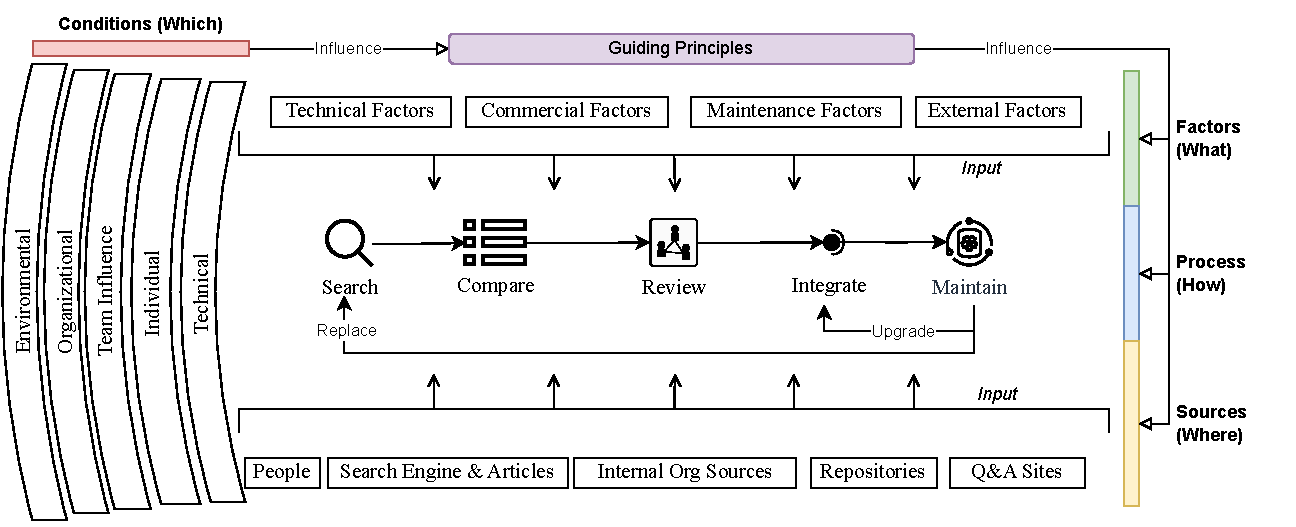
\includegraphics[scale=0.85]{images/Library-adoption-framework.v3.pdf}
    \caption{Conceptual framework of the software library adoption model}
    \label{fig:framework}
\end{figure*}















%\begin{figure*}
%    \centering
%    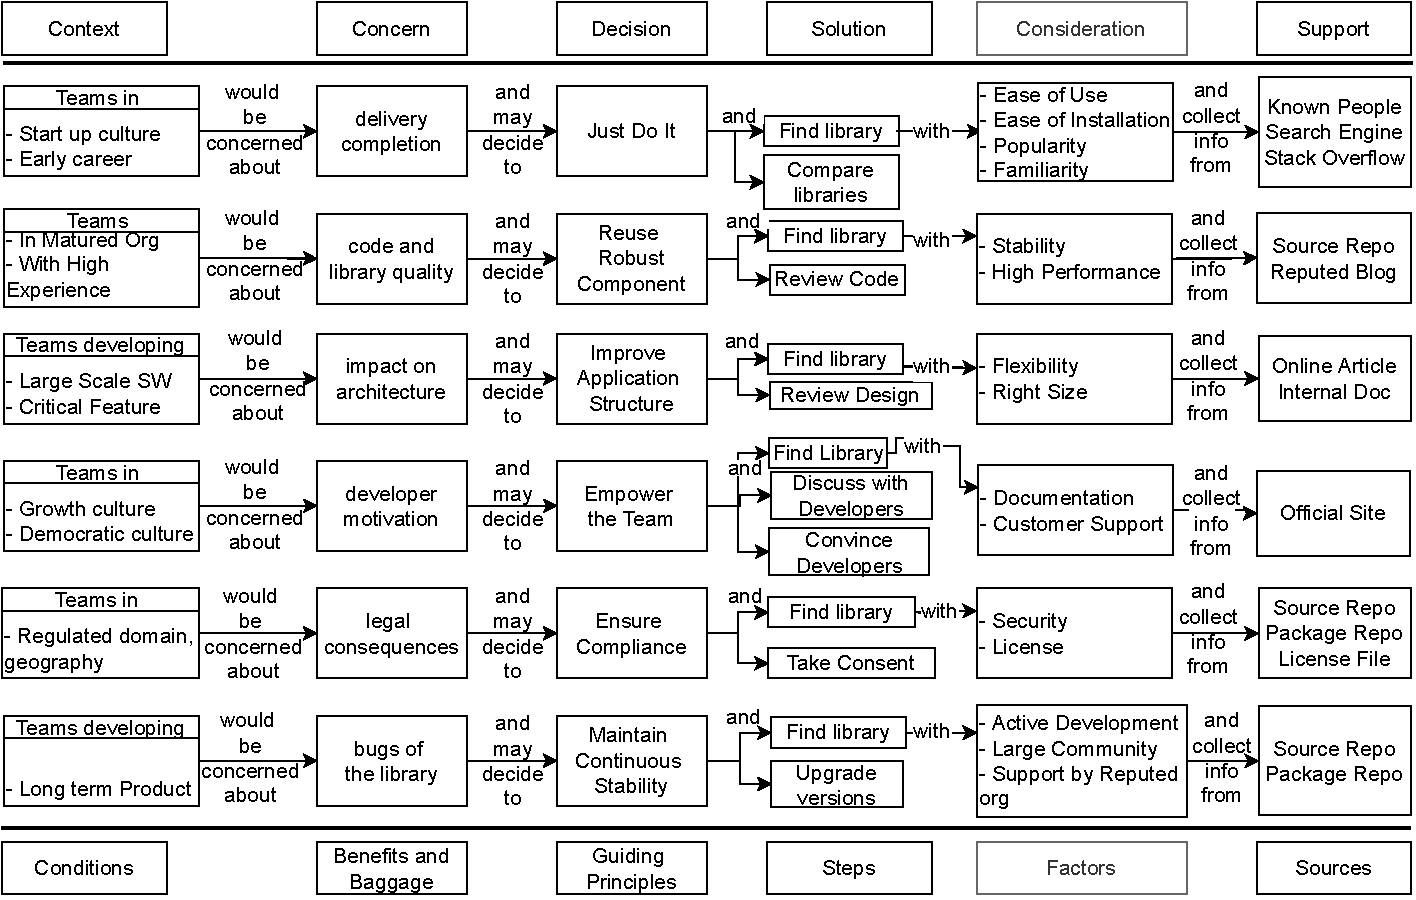
\includegraphics[scale=0.75]{images/gp-concepts-2.pdf}
%    \caption{Interaction of guiding principles with library adoption life cycle %concepts according to the conceptual framework}
%    \label{fig:gp-scneraios}
%\end{figure*}







%\section{Guiding Principles and Life Cycle of Library Adoption}
%\label{sec:taxonomy}
%\begin{figure*}
%    \centering
%    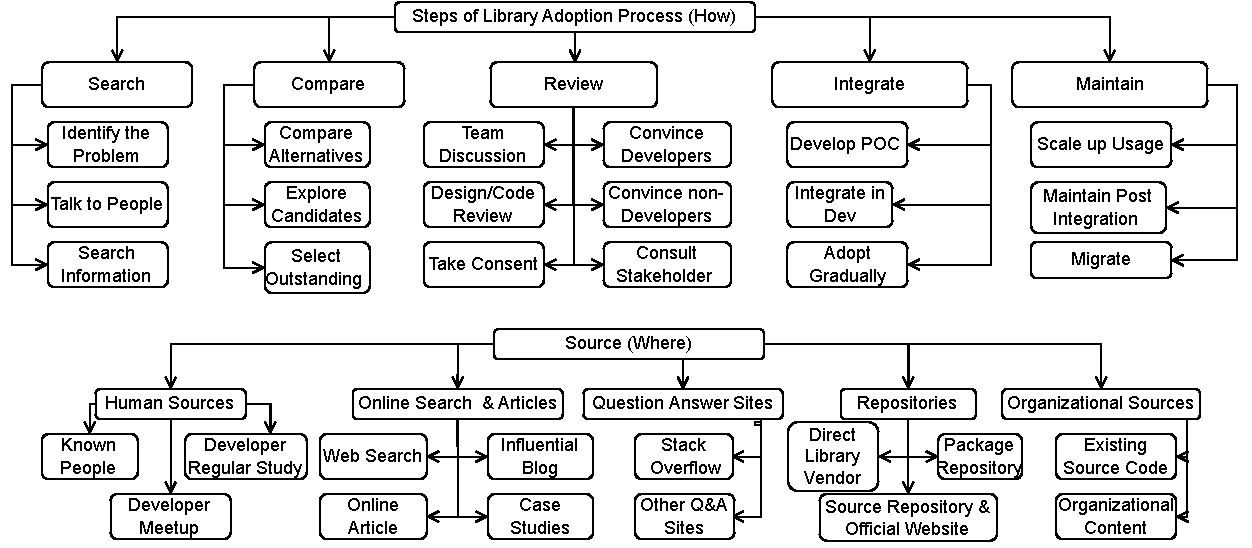
\includegraphics[scale=0.85]{images/process.pdf}
%    \caption{Concepts related with library adoption process and relevant information sources}
%    \label{fig:process}
%\end{figure*}
% Using open coding and constant comparison of \td{24} interviews, we discovered total 83 library adoption concepts. By conducting axial coding, we categorized these concepts into 19 categories under 4 major categories of adoption steps, surrounding conditions, library specific factors, and information sources. Figure \ref{fig:taxonomy} shows the hierarchy of all 83 library adoption concepts. Numbers shown beside the major categories in Figure \ref{fig:taxonomy} refer to the total number of concepts under that category (e.g., 18 concepts under 'steps' category).


\subsubsection{Steps of Library Adoption (L)}\label{sec:phases} 

% [Minaoar] I assumed it was deleted mistakenly and added it back.
%% Ann: Nope, deleted on purpose. We have to tell one story well and not get bogged down in details.
%\begin{figure*}
%   \centering
%   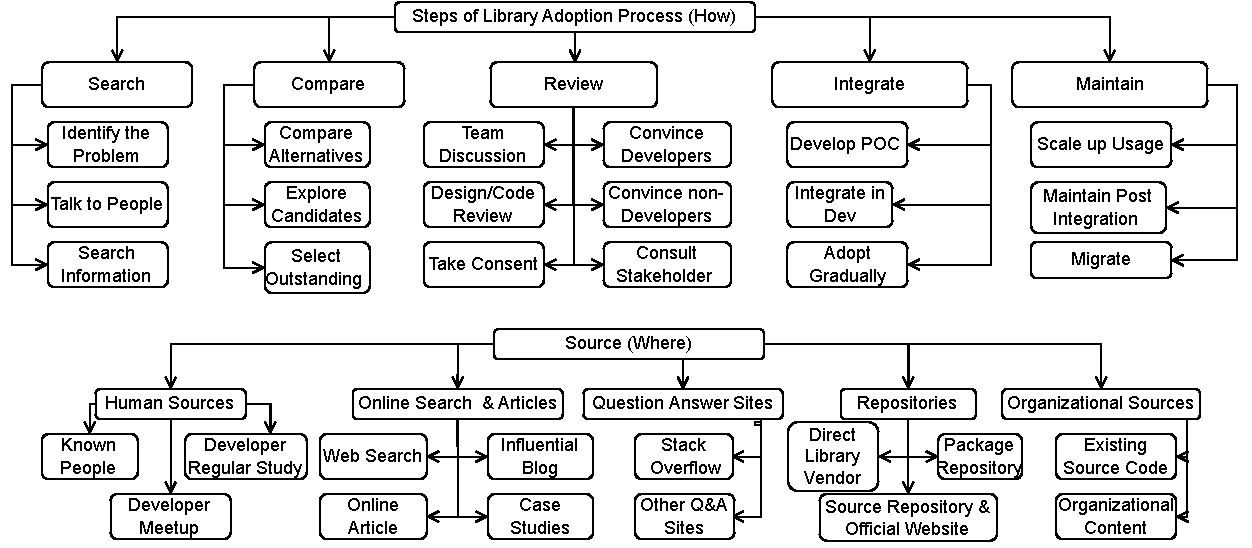
\includegraphics[scale=0.85]{images/process.pdf}
%   \caption{Concepts related with steps library adoption process}
%   \label{fig:process}
%\end{figure*}

The adoption of a third-party library consists of five steps, as depicted in the `Process' section of Figure~\ref{fig:framework}. The steps are: search for library information, compare available libraries, review libraries along with other teammates or teams, integrate the library into the application, and maintain the library through the life cycle of the host application. There were 18 concepts associated with \code{steps of library adoption process} in our code system. Figure~\ref{fig:process} in the Appendix shows the relationship between relevant codes and categories.

\code{Search} entails \code{identifying the problem}, \code{talking to people}, and \code{performing an online search}. Next, developers \code{compare} available libraries by \code{comparing alternatives}, \code{exploring candidates}, and \code{selecting the outstanding library}. The comparison concept is explained by P15:

\qi{You go to Stack Overflow and you find some articles there that refers to some of the libraries. From there you go into those libraries spaces and GitHub and then you take a look at it.}{P15} 

\code{Review} of the library can involve multiple concepts: \code{team discussion}, \code{design/code review}, \code{consent process}, \code{convince developers}, \code{convince non-developers}, and \code{stakeholder consultation}. Depending on the company size and practices, developers may request approval from dedicated teams who review the security and license issues of third party libraries: 
\qi{So we have the DevOps team\ldots they have a way to check the security also any vulnerability issue altogether and also if we are actually using it in the proper license.}{P11} 


To \code{integrate} a library can also be a gradual process, consisting of \code{proof of concept development}, \code{integration}, and \code{gradual adoption}, as illustrated here:
\qi{[We] do some proof of concept for some libraries. Then for the adoption phase we normally take it slowly, like for example, when we want to introduce Hikary CP instead of Tomcat, we have to apply this library to one or two services, then gradually move to the wide adoption of that library.}{P01} 

Finally, to \code{maintain}, developers may \code{scale up usage}, perform \code{post integration maintenance}, and \code{migration}. Once the code has been included, developers may need to keep up with the latest versions:

\qi{There is no limit on improvement\ldots You can opt in for new 
versions or you can ignore the new versions. Usually major versions might have something which can break your code. But you don’t upgrade without any reason.}{P05}
%\todo{@Minaoar - I took this quote from elsewhere, please replace it if it isn't coded under maintain} \minaoar{looks good}.


\subsubsection{Source of Information about Libraries (S)} \label{sec:sources}
Developers seek out information about libraries from a variety of sources when making an evaluation, as shown in Figure~\ref{fig:framework}. The main categories of information \code{source} are \code{human sources}, \code{online search and articles}, \code{question answer sites}, \code{repositories}, and \code{organizational sources} internal to the company. Within these five categories, we identified 14 concepts, whose hierarchical relationship is shown in Figure~5 of the Appendix.

Of the \code{human sources} available to developers, there are \code{known people}, the developer's \code{regular study}, and \code{developer meetup}. Which sources the developer favors can vary, as illustrated by these two quotes:
\qi{The first thing is not opinion from other people, rather from developer's daily study. Developers always look for [learning] things, right?}{P01}
\qi{The very first step before going to searching is I'm reaching out to my colleagues.}{P11}

For \code{online search and articles}, developers can turn to \code{web search}, \code{online article}, \code{influential blog}, and \code{case studies}. Alternately, they may turn to \code{question and answer sites} such as \code{Stack Overflow} or \code{other Q\&A sites}. The value of question and answer sites as a source of information is described by P07:
\qi{Stack Overflow is a huge resource for seeing what different people recommend\ldots and also seen a lot on things like Quora and Reddit where you say what's the best library for doing X and people will list out a couple of different options there.}{P07}

Another source of information is \code{repositories}, which can consist of the \code{direct library vendor},\code{package repository}, or \code{source repository and offical website}. Finally, developers can turn to internal \code{organizational sources}, namely \code{existing source code} and \code{organizational content}. As one respondent explained,
\qi{[We have an] internal GitHub. Then there are internal search engines, also there are some question answer like Stack Overflow\code I think that is true for all these big corporations.}{P02}


\subsection{Factors and Conditions influencing Life Cycle (RQ2)}

Our second research question was ``What conditions and technical factors influence the library adoption process?'' In order to answer this question, we turn to the conditions of library adoption and the factors of library selection criteria.

\subsubsection{Conditions of Library Adoption (C)}\label{sec:conditions}
Library adoption life cycle can be influenced by environmental, organizational, team specific, individual, and technical scenario specific conditions and opinions. These conditions affect which guiding principles are most appropriate. In the major category of \code{conditions}, we identified five categories: \code{environmental}, \code{organizational}, \code{team influence}, \code{individual}, and \code{technical}, which are depicted in relation to the life cycle of adoption in Figure~\ref{fig:framework}. There were 23 concepts associated with these categories, as shown on Figure~\ref{fig:conditions} in the Appendix.

\code{Environmental} conditions include the \code{geographic} and \code{legal} landscapes. For example, regulatory requirements influence the legal conditions under which the company operates:
\qi{in Germany you have to report a security breach in your company\ldots you have to pay two percent of the revenue if a security breach happens and your data gets leaked.}{P17} 
Geography, too, can influence selection, outside of any legal requirements:
\qi{{\ldots} everywhere it's not still functional programming, it's not widely adopted. I recently migrated from Asia to Europe and I never saw this trend widely adopted in our previous the companies. But here [in Europe], I've seen a lot of people are very interested about that functional programming paradigms. So, to choose the libraries, maybe their background, their geography, their location, that all of these things can have some impact.}{P01}

Organizations can also enforce policies for library selection. Under \code{organizational} conditions we observed \code{investment capacity}, \code{company culture}, existing \code{company tech}, and \code{application domain}. There can also be a \code{team influence}, based on \code{team capability}, \code{expert/lead opinion}, \code{operations opinion}, \code{peer opinion}, \code{stakeholder opinion}, and \code{product/project manager opinion}. Team capability is demonstrated with the following quote:
\qi{I went for Vue because most of the developers in my company were mostly back-end developers and I found Vue is very back-end developer friendly.}{P04}

\code{Individual} developers can also have personal characteristics which are independent of technology but which influence library selection. These can include \code{personal background}, \code{personal motivation}, and \code{experience level}. An example of personal motivation is:
 \qi{The excitement of trying some new library was also fairly motivating to keep my skills up to date\ldots}{P06} 

 Finally, there can be \code{technical} conditions, namely a severe issue in production (\code{stuck in production}), having a \code{tight deadline}, \code{migration to a different library}, \code{criticality of feature}, \code{new feature}, \code{tech stack upgrade}, \code{library upgrade}, and \code{OS upgrade}. The influence of criticality can be seen here:
\qi{If the feature is too business critical, then it goes through even rigorous decision making process than the other where, for example, you are just trying to choose a library to show an image and crop it. So that is not so business critical.}{P15}



\subsubsection{Factors of Library Selection Criteria (F)}\label{sec:factors}
The factors of the library itself help inform the life cycle, as depicted in Figure~\ref{fig:framework}. We identified four categories of \code{factors}: \code{software factors}, \code{commercial factors}, \code{maintenance factors}, and \code{external factors}. Under these we found 28 concepts, whose relation to the categories is shown in Figure~6 in the Appendix.

In the category of technical \code{software factors}, we see \code{compatibility}, \code{stability}, \code{flexibility}, \code{capability}, \code{security}, \code{performance}, \code{ease of use}, \code{ease of installation}, \code{size of library}, and \code{interesting interface} as concerns. Several of these considerations are provided by P15:
\qi{We have to understand how much memory it is gonna use. How much time it takes to execute? Or how much CPU is gonna use? Is this library compatible with the development environment? How is the thread safety within the library?}{P15}

After technical factors, developers may have to consider \code{commercial factors} such as \code{license}, \code{cost}, \code{dependency}, \code{roadmap}, \code{open source}, \code{documentation}, and \code{demo availability}. An example of the impact of demo availability on the selection process is:
\qi{And one thing I prefer over other GitHub repository is that if it has a working demo available on the web. For example, if it is a front end library, then it has a UI. If it's a back end library, it has some kind of documentation available like Swagger so that I can make a call to the library and see how it works. If some kind of live demo available, then I feel more confident about it.}{P15}

\code{Maintenance factors} include whether the code is under \code{active development}, enjoys \code{community support}, is \code{supported by a reputed organization}, has a \code{large community}, offers \code{customer support}, and is \code{supported by own organization}. 

Finally, \code{external factors} can come into play. These include \code{popularity}, \code{search engine ranking}, \code{familiarity}, \code{used by reputed organizations}, and \code{detailed benchmark}. The following quotations demonstrate how popularity and familiarity affect selection:
\qi{We cannot compare sixty million with one thousand downloads. So this library [with high download count] is obviously a choice.}{P04} 
 \qi{Oftentimes what happens is that the decision or the choice gets influenced by individual's bias or familiarity or previous experience with one particular product or service}{P08} 


\subsection{Guiding Principles (RQ3)}
\label{sec:gp}

All of the concepts of the library adoption life cycle described in section \ref{sec:framework} have complex interactions which are captured in the six guiding principles.  The guiding principles have all the characteristics of patterns; that is, they represent an abstract solution to a recurring problem \cite{riehle:2021:pattern}. On the basis of internal and external conditions \qww{C}, certain advantages and disadvantages of libraries become relevant to developers, and they follow a guiding principle accordingly. The choice of guiding principle then influences the selection factors \qww{F}, information sources \qww{S}, and finally the steps toward adoption \qww{P}. As one participant explained,
 \qi{It's not that always you have to choose a library or framework which is technically the best. Rather capabilities of the library and the organization, the domain, the people, the timing, everything influences that decision.}{P01} 

It must be noted that conditions do not come in isolation, and guiding principles also do not activate exclusively. Rather, in practical scenarios, developers are always facing multiple, even conflicting situations, and are balancing between guiding principles to make their final decisions.

Due to space limitations, we are only able to present some of the guiding principles in depth. All six can be found in the Appendix.


%%%%%%% GP 1
\subsubsection{GP1: Just Do It}
When developers are concerned primarily with time-to-market, or are not that interested in long-term maintenance, they may opt to make use of a third-party libraries which are \qqw{F}{easy to use} and \qqw{F}{easy to install}, as illustrated by the following quotes. 
% \begin{practice}{1}{Just Do It}
\actor{Developers}
\condition{Faster go to market is critical. Developers rewarded for delivering minimum feature on time.}
\concern{How the developers can meet the deadline with relatively less effort?}
\solution{Use a third-party library that reduces the work load and delivery can be done on time}
\consideration{Easy to use, easy to install, popular, and familiar library.}
\steps{Find libraries, compare them, and choose one according to the consideration. Take support from known people or use search engine or Stack Overflow}
\consequence{Can lead to future maintenance burden such as performance bottleneck or security vulnerability.}
\example{For startups, a lot of it [priority] is just speed to market and how much resources is gonna eat up using any specific library.}{P07}
\end{practice}

% \begin{table}[]
%     \centering
%     \caption{Scenario of GP1: Just Do It}
%     \begin{tabular}{p{1cm}p{6.5cm}}
%          \toprule
%             \textbf{GP} & \textbf{Just Do It} \\ 
%             \midrule
%             Actor(s) & Developers \\ 
%             Context & - Faster go to market is critical for business. Developers are often rewarded for delivering minimum viable product on time.
%             - Developers are in their early career and assume higher satisfaction on faster delivery. \\ 
%             Concern & How the developers can meet the deadline in relatively less effort? \\ 
%             Solution & Use a third-party library that reduces the work load and delivery can be done on time \\ 
%             Consider-ation & The library should be easy to use, easy to install, popular, and even better if developer is already familiar with it. \\ 
%             Steps & Find libraries, compare them, and choose one according to the consideration \\ 
%             Support & Take support from known people to know about such library or use search engine, Stack Overflow \\ 
%             Example Trace in Data & For startups, a lot of it [priority] is just speed to market and how much resources is gonna eat up using any specific library. (P07) \\ 
%          \bottomrule
%     \end{tabular}
%     \label{tab:gp1-scenario}
% \end{table}
 

\qi{[The library] makes our life simpler. The application development definitely gets faster by using that.}{P15}
\qi{It was going to solve a particular promotion or something, and it was going to be retired. So usually the long term maintainability was not a factor.}{P06}



%%%%%%%% GP 2
\subsubsection{GP2: Reuse Robust Component}
Developers working on long-term or complex products prefer to choose \qqw{F}{stable} which are \qqw{F}{actively maintained} for a long period and supported by a \qqw{F}{large community}. The guiding principle is ``Reuse Robust Component.'' Examples of its use are:

\qi{Don't reinvent the wheel. I want to use as much as already developed, tested and robust software into my solution\ldots the main thing is that reusability and having stability in the application inherently out-of-the-box by using a stable, robust library}{P22}
\qi{With a project like ours [C++ code application developed over 27 years], the main time we adopt a library is when it is an implementation of a tech spec. OpenSSL, there's a tech spec for SSL. Here's a whole library that has been carefully implemented against the spec.}{P18}

%\begin{practice}{2}{Reuse Robust Component}
\actor{Developers, Senior Developers}
\condition{Mature organization, stable code. Developers concerned of quality, performance \& maintainability.}
\concern{How can the application avoid boiler plate code and follow best design principles?}
\solution{Use a trusted proven third-party library that will keep the code clean and manageable.}
\consideration{Open source, community trusted, stable and high-performing library.}
\steps{Find and compare libraries, review thoroughly by more than one developer. Look into the library's source code repository to analyze the stability, quality of the library, and also consider reputed technical blogs.}
\consequence{Too much analysis and exploration can be an overkill for small features causing delivery delay.}
%\hline
\example{So [this large corporation] as a whole is actually built on the open source libraries that are suitable for our use cases. But that actually has been one of our primary focus as well. If you find a library, use it; only build if you can’t find anything.}{P13}
\end{practice}

% \begin{table}[]
%     \centering
%     \caption{Scenario of GP2: Reuse Robust Component}
%     \begin{tabular}{p{1cm}p{7.5cm}}
%          \toprule
%             \textbf{GP} & \textbf{Reuse Robust Component} \\ 
%             \midrule
%             Actor(s) & Developers, Senior Developers \\ 
%             Context & - Matured organization with stable source code and release pipeline. Application performance and maintainability is a big concern for the team.
%             - Developers with higher experience would be careful about the quality of the application source code. \\ 
%             Concern & How the application can avoid boiler plate code and follow best design principles? \\ 
%             Solution & Use a trusted proven third-party library that will keep the code clean and manageable. \\ 
%             Consider-ation & The library should be open source, trusted by community, stable and provide apppropriate performance metrics required \\ 
%             Steps & Find and compare libraries, review thoroughly by more than one developer. \\ 
%             Support & Look into the library's source code repository to analyze the stability, quality of the library, and also consider reputed technical blogs. \\ 
%             Example Trace in Data & So [this large corporation] as a whole is actually built on the open source libraries that are suitable for our use cases. But that actually has been one of our primary focus as well. If you find a library, use it; only build if you can’t find anything. (P13) \\ 
%          \bottomrule
%     \end{tabular}
%     \label{tab:gp2-scenario}
% \end{table}
 %% Ann: I exclude this one because it is fairly evident (to save space)

%%%%%%% GP 3
\subsubsection{GP3: Maximize Flexibility}
%\vspace{-5mm}
\begin{practice}{3}{Maximize Flexibility} % Was Improve Application Structure
\actor{Developers, Architects}
\condition{Large scale software applications have their own structure which evolved over time and may follow some software design principles. System designers want to use new libraries in a way that improves the application structure, or at least does not deteriorate it.}
\concern{How can the architecture be improved or be protected from unwanted rigidity while using a library?}
\solution{Use a library that just fits right with the application in terms of the size and flexibility. Consider wrapping the third-party library in an API to allow replacement of the library without affecting dependent code.}
\consideration{The library should be flexible and should not be too large in size compared to the system.}
\steps{Find, compare, and review libraries. Conduct design review to assess impact on architecture. Review internal organizational content for design principles.}
\example{The moment you have to bring something in because there are new requirements is the time to assess how you've structured your application and does it still serve you and your customers or the business requirements you have. So that’s the opportunity to look at the structural aspect of the application and make sure you do want to avoid changing it or maybe
it's the time to change it.}{P22}
\end{practice}%\vspace{-4mm}

% \begin{table}[h]
%     \centering
%     %\caption{Scenario of GP3: Maximize Flexibility}
%     \begin{tabular}{p{8.5cm}}%{p{1cm}p{7.5cm}}
%          \toprule
%          \textbf{Guiding Principle 3 - Maximize Flexibility} \\% & \textbf{Improve Application Structure} \\ 
%          \midrule
%             \bf{Actor(s).} Developers, Architects \\ %\midrule 
%             \bf{Condition.} Large scale software applications have their own structure which evolved over time and may follow some software design principles. System designers want to use new libraries in a way that improves the application structure, or at least does not deteriorate it.\\ %\midrule 
%             \bf{Concern.} How can the architecture be improved or be protected from unwanted rigidity while using a library?\\ %\midrule 
%             \bf{Solution.} Use a library that just fits right with the application in terms of the size and flexibility. Consider wrapping the third-party library in an API to allow replacement of the library without affecting dependent code.\\ %\midrule 
%             \bf{Consideration}. The library should be flexible and should not be too large in size compared to the system.\\ %\midrule 
%             \bf{Steps.} Find, compare, and review libraries. Conduct design review to assess impact on architecture. Review internal organizational content for design principles.\\ %\midrule 
%             \bf{Example}. \emph{``The moment you have to bring something in because there are new requirements is the time to assess how you've structured your application and does it still serve you and your customers or the business requirements you have. So that’s the opportunity to look at the structural aspect of the application and make sure you do want to avoid changing it or maybe it's the time to change it."}{P22} \\ 

%          \bottomrule
%     \end{tabular}
%     \label{tab:gp3-scenario}
% \end{table}
 
While inspired by the principle of architectural improvement and consistency, architects adopt third party libraries when absolute necessary for specifications. The project P18 worked was such an example where they had less than 20 libraries in a two million line source code. Even when they \qqw{P}{integrate} libraries, they would wrap it under their own structure: 
\qi{We will create just a thin wrapper, that ends up looking like the rest of our platform. The simple source file [wrapper API] is protecting the two million lines of code from the idiosyncrasies of this one particular library.}{P18}
\qi{Just go with the smaller libraries that solve a very particular problem so that we have full control. But if we integrate with the framework then we always need to solve with that framework because we cannot go outside of that framework until we completely remove that framework}{P9}



%% GP 4
\subsubsection{GP4: Empower the Team}
Adopting third party libraries also empowers the development teams. Open source libraries provide developers working experience with popular development components to acquire transferable knowledge whereas proprietary solutions developed internally can create bottlenecks: 
\qi{When you move to using something that's an open source third party solution, it's well documented, suddenly an entire team of people can help address a problem and your speed to fixing something goes from multiple days or weeks to hours. And you empower the whole team rather than an [internal] specialist who can't go on vacation because if she does, sorry, you're waiting.}{P22}

 When guided by the empowerment principle, developers often consider \qqw{C}{peer opinions} during the library \qqw{P}{review} phase: 
 \qi{Let's say, I proposed one library from my previous work. And then I have to explain it to the team members.}{P10}
 \qi{I'm not taking a decision for myself. Also there are seniors in every organization who are more experienced and they may have some opinions on it.}{P01}

%\vspace{-5mm}
\begin{practice}{4}{Empower the Team}
\actor{Developers, Tech Leaders}
\condition{Strong company culture to promote transferable skill and provide learning space for developers. 
%Tech leaders may care more for their team's capacity, limitations, and motivations.
The development team may have limitations or strengths in certain technologies. }
\concern{Does the library fit well within the capability of the dev team? Will it provide any transferable skills?}
\solution{Use a library appreciated by the developers}
\consideration{Well documented, popular, easy to use library with customer support.}
\steps{Besides finding a library that fits well with the technology, thoroughly discuss with developers about their opinion and acceptance of the library. Look into official documentation of the library.}
\consequence{May compromise the optimum technology for dev team's limitation. Can keep teams motivated.}
\example{So looking at community popularity helps because then it helps to hire people. It helps to retain people. They like to use technologies that are transferable.}{P19}
\end{practice}%\vspace{-4mm}


% \begin{table}[]
%     \centering
%     \caption{Scenario of GP4: Empower the Team}
%     \begin{tabular}{p{1cm}p{7.5cm}}
%          \toprule
%             \textbf{GP} & \textbf{Empower the Team} \\ 
%             \midrule
%             Actor(s) & Developers, Tech Leaders \\ 
%             Context & - Some organizations may have strong company culture to improve development skill set or for providing comfortable learning space for developers. 
%             - Tech leaders may care more for their team's capacity, limiatation, and motivation.
%             - Development team may have limitation or strength in certain technology  \\ 
%             Concern & Does the library fit well with the capability of the development team? Will it provide them any transferable skill? \\ 
%             Solution & Use a library that is appreciated by the developers \\ 
%             Consider-ation & Library should be well documented, should be community popular so that developers can easily adopt and can refer in future. Also it can have customer support in case developers needs extra help. \\ 
%             Steps & Besides finding a library that fits well with the technology, thoroughly discuss with developers about their opinion and acceptance of the library. \\ 
%             Support & Look into official documentation of the library for documentation and support issues. \\ 
%             Example Trace in Data & So looking at community popularity helps because then you can it helps to hire people. It helps to retain people. They like to use technologies that are transferable (P19) \\ 
%          \bottomrule
%     \end{tabular}
%     \label{tab:gp4-scenario}
% \end{table}
 %% Ann: I include this one because it is not something most people consider

%% GP 5
\subsubsection{GP5: Ensure Compliance}
Third-party libraries can come with licensing issues, privacy concerns, or security vulnerabilities.
However, not all development teams equally consider the impact of compliance issues. \qqw{C}{Legal environment} of the organization or their customers are primary driver for compliance principle: 
\qi{Since we work with people from Europe, UK, US and other areas and they have a very strong data security policy, we have to be confident that they're secure well.}{P04} 
\qi{So there are libraries who advertise that they are already GDPR \cite{website:gdpr} compliant or FedRAMP \cite{website:fedramp} compliant. So those kinds of libraries are always preferred over libraries that don't have a clear signal.}{P19} 

%\begin{practice}{5}{Ensure Compliance}
\actor{Developers, Information Security Experts, Legal Experts, Open Source Program Office}
\condition{Because of regulatory compliance or for company culture, some organizations will be more cautious about using third-party libraries for legal, security, and privacy reasons. 
Developers will often have little technical expertise on such specialized issues.
Sometimes small or early stage companies may even ignore the importance of compliance issues.
A few application domains such as health, finance, media are also more regulated and require organizational policies for ensuring compliance.}
\concern{Will there be any penalty or legal complication arising from using a third-party library? How to protect the organization?}
\solution{Use a library which is compliant with the application security standards and legal requirements}
\consideration{The license of the library should be compatible with the business and license of the target software. The security and privacy concerns should be clarified and well taken care of by the library contributors.}
\steps{Reach out to specialists in the organization for taking their expert consent before adopting the library. See the license and security declarations in the library documentation in the source code or package repository.}
\example{We had a very bad experience with this. With the legacy system, we were using so many different libraries and there is a licensing issue and we had to replace half of the library. Otherwise we had to pay lots of money. So that's why we are now very, very concerned about adding any external library, because if we don’t comply with the license, it will be a legal problem.}{P09}
\end{practice}

% \begin{table}[]
%     \centering
%     \caption{Scenario of GP5: Ensure Compliance}
%     \begin{tabular}{p{1cm}p{7.5cm}}
%          \toprule
%             \textbf{GP} & \textbf{Ensure Compliance} \\ 
%             \midrule
%             Actor(s) & Developers, Information Security Experts, Legal Experts, Open Source Program Office \\ 
%             Context & - Because of regulatory compliance or for company culture, some organizations will be more cautious about using third-party libraries for legal, security, and privacy reasons. 
%             - Developers will often have little technical expertise on such speialized issues
%             - Sometimes small or early stage companies may even ignore the importance of compliance issues
%             - Few application domains such as health, finance, media are also more regulated and require organizational policies for ensuring compliance. \\ 
%             Concern & Will there be any penalty or legal complication arising from using a third-party library? How to protect the organization? \\ 
%             Solution & Use a library which is compliant with the application security standards and legal requirements \\ 
%             Consider-ation & License of the library should be compatible with the business and license of the target software. The security and privacy concerns should be clarified and well take care of by the library contributors. \\ 
%             Steps & Reach out to specialists in the organization for taking their expert consent before adopting the library. \\ 
%             Support & See the license and security declarations in the library documentation in the source code or package repository. \\ 
%             Example Trace in Data & we had a very bad experience with this. With the legacy system, we were using so many different libraries and there is a licensing issue and we had to replace half of the library. Otherwise we had to pay lots of money. So that’s why we are now very, very concerned about adding any external library, because if we don’t comply with the license, it will be a legal problem. (P09) \\ 
%          \bottomrule
%     \end{tabular}
%     \label{tab:gp5-scenario}
% \end{table}
 %% Ann: I exclude this one because it is fairly evident (to save space)

%% GP 6
\subsubsection{GP6: Maintain Continuous Stability}
Aside from compliance issues, the biggest risk of using a third-party library is that the library won't be maintained.

\qi{If the contributors are gone in those third party libraries repositories, suddenly the whole production application is broken}{P10} 

To protect themselves from abandonment and stability risks, developers look for libraries where a \qqw{F}{large community} and contributors are involved. To \qqw{P}{search information} about \qqw{F}{active development}, they check \qqw{S}{source repositories}: 
\qi{We have to check that whether this library maintenance are active or not. We can determine that by checking their GitHub repository when was the last push was given?}{P04} 

% \begin{practice}{6}{Maintain Continuous Stability}
\actor{Developers, DevOps}
\condition{Some software applications are developed and maintained for long term. A third-party library used in such a product can have bugs or vulnerabilities that need to be fixed. Sometimes, the contributors of the library may not continue to fix bugs or improve with new features. Sometimes libraries may not have backwards compatibility and when developers upgrade, their existing system can break.}
\concern{How will developers ensure that a library is well maintained in foreseeable future and that they can keep using the library without breaking their application?}
\solution{Use a library with good history of maintenance and prepare to continuously upgrade the library in future}
\consideration{Selected libraries should be actively maintained by contributors, supported by reputed organizations, and have larger community.}
\steps{Analyze the maintenance and issue history of the library to assess the active development practices or the library. Establish a process for software bill of materials to document all third-party library dependencies and their upgrade plan in conjunction with DevOps teams. Look into source code commit and issue history from source repository and download usage trend from package repository.}
\example{When we integrated the updated version our whole interface broke. And we had to change a lot of code, all the interceptors, interfaces, everything\ldots This maintenance is quite hard. It's actually a full time work to always keep updated, to always stay updated.}{P14}
\end{practice}

% \begin{table}[]
%     \centering
%     \caption{Scenario of GP6: Maintain Continuous Stability}
%     \begin{tabular}{p{1cm}p{7.5cm}}
%          \toprule
%             \textbf{GP} & \textbf{Maintain Continuous Stability} \\
%             \midrule
%             Actor(s) & Developers, DevOps \\ 
%             Context & - Some software applications are developed and maintained for long term. A third-party library used in such a product can have bugs or vulnerabilities that need to be fixed. Sometimes, the contributors of the library may not continue to fix bugs or improve with new features. Sometimes libraries may not have backwards compatibility and when developers upgrade, their existing system can break. \\ 
%             Concern & How developers will ensure that a library is well maintained in foreseeable future and can keep using the library without breaking their application? \\ 
%             Solution & Use a library with good history of maintenance and prepare to continuously upgrade the library in future \\ 
%             Consider-ation & Selected libraries should be actively maintained by contributors, supported by reputed organizations, and have larger community. \\ 
%             Steps & Analyze the maintenance and issue history of the library to assess the active development practices or the library. Establish a process for software bill of materials to document all third-party library dependencies and their upgrade plan in conjunction with DevOps teams. \\ 
%             Support & Look into source code commit and issue history from source repository and download usage trend from package repository. \\ 
%             Example Trace in Data & when we integrated the updated version our whole interface broke. And we had to change a lot of code, all the interceptors, interfaces, everything... This maintenance is quite hard. It’s actually a full time work to always keep updated, to always stay updated. (P14) \\ 
%          \bottomrule
%     \end{tabular}
%     \label{tab:gp6-scenario}
% \end{table}
 %% Ann - excluded to save space


% During the theoretical integration of our study, the six guiding principles emerged from the benefits and baggage of libraries - why developers want to use a library and why they still remain cautious to use a library.














%\section{Proof of Concept for Future Research}
\section{Needs for Tool Support to Support Third-Party Software Library Adoption (RQ2)}
We discovered from the barriers developers face in the library adoption process that besides organizational limitations, developers are also impacted by the lack of selection tools. Hence, during our qualitative study, we also came up with potential solution proposals for selection tools and evaluated the usability of those solutions. We also collected feedback from our interviewees through an additional survey on the latest technology tools like ChatGPT and its potential usage in library selection.

In this section, we will explore two potential library selection tools along with their motivation and industry evaluation. We shall also present a default priority score of selection factors that can be used by any library selection tool.

\subsection{Library Selection using a Conceptual Tool}
We conceptualized a library selection tool combining the findings of our qualitative research and marketing theories.
\subsubsection{Concept Development from Marketing Model on Buyer Behavior}
During our interview analysis, we found that our \model\space is similar to consumer and business buyer behavior models and decision process of marketing theories \cite{kotler2014principles}. The exact comparison of the models and the buying decision and adoption processes are shown in Figure \ref{fig:model-comparison} and in Figure \ref{fig:process-comparison}.

\begin{figure*}
    \centering
    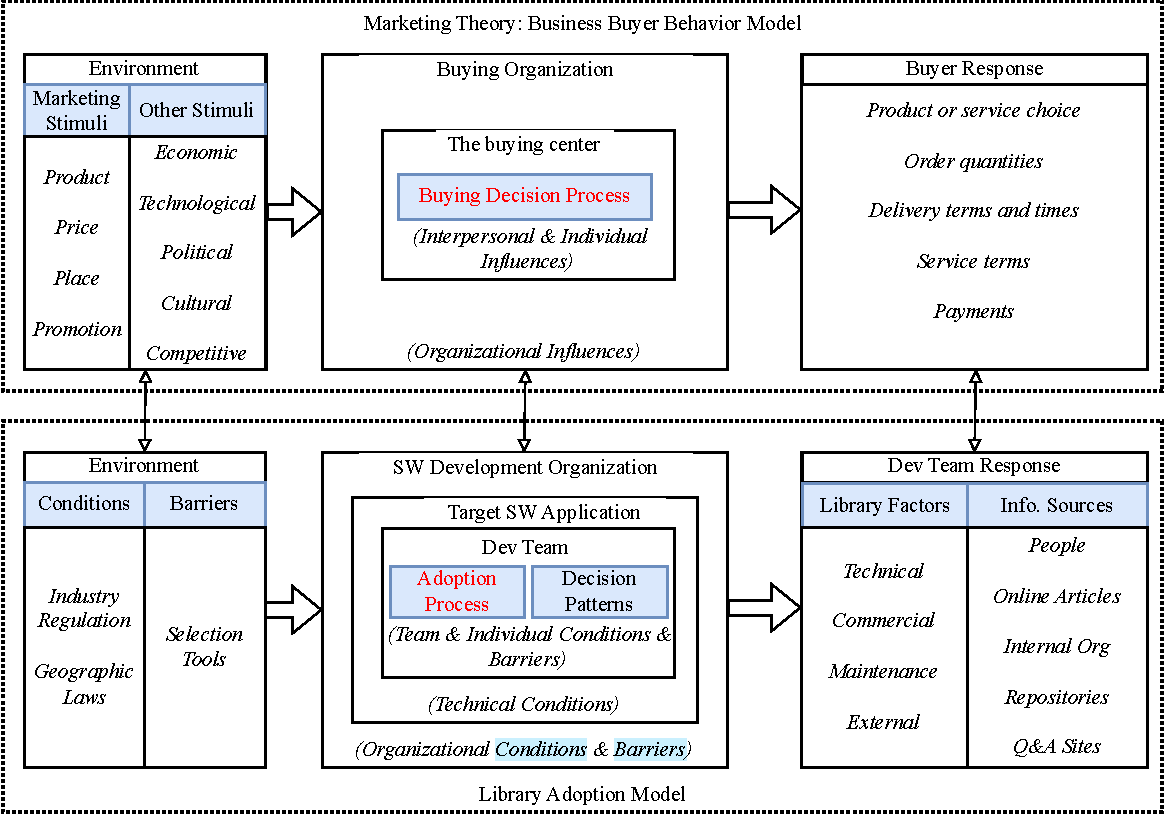
\includegraphics[scale=0.8]{images/Buyer-behavior-models-comparison.pdf}
    \caption{Similarity between \model\space and business buyer behavior model redrawn verbatim from marketing theories \cite{kotler2014principles}. The similar blocks between the two models are mapped using the arrow. While the major building blocks of the two models are identical, in addition to the marketing model, we found \principle\space, challenges, and technical conditions in the \model.}
    \label{fig:model-comparison}
\end{figure*}

\begin{figure*}
    \centering
    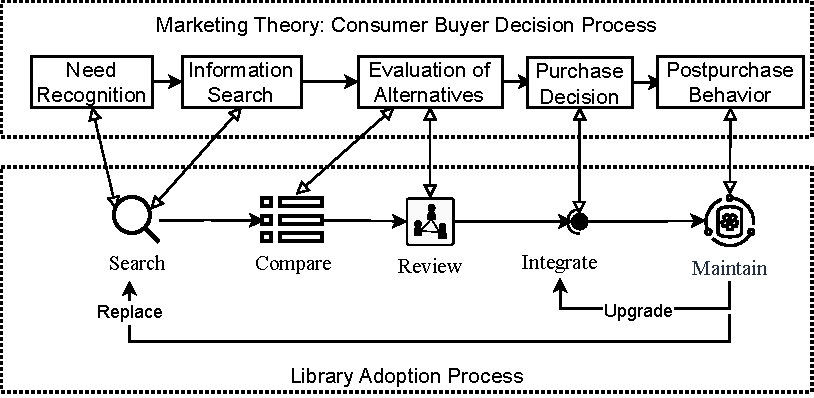
\includegraphics[scale=.8]{images/Decision-adoption-process-comparison.pdf}
    \caption{Similarity between consumer buyer decision process redrawn verbatim from marketing theories \cite{kotler2014principles} and library adoption process. The similar steps between the two processes are mapped using the arrow.}
    \label{fig:process-comparison}
\end{figure*}

The adoption conditions in our model match with business/organization buyer behavior conditions. The two models are also similar in terms of actors. However, unlike the business buying behavior model which has supplier search, selection, and performance review for the traditional procurement process, the library adoption process is simpler and closely relates with the consumer buying behavior. The consumer buying process has need recognition, information search, alternative evaluation, purchase decision, and post-purchase behavior. In our \model, we have split the purchase decision to \code{review} (where most decision is taken) and \code{integrate} steps and merged \code{problem identification} under \code{search} step. Since \model\space resembles the consumer buyer behavior process, it also opens up opportunities to utilize further marketing models in the library adoption process. For example, if Fishbein Multiattribute Model \cite{fishbein1967attitude} can be applied to the consumer model, it can also be applied to the library adoption model. In Multiattribute Model, two products can be compared based on certain factors (f). Each factor has an associated weight (w). The consumer assumes a certain score (s) for each product based on every factor and calculates a net score (NS) by computing the weighted average of the factor scores (s) and weights (w). For example, if there are n factors for a product (P), then the net score (NS) according to Multiattribute Model is calculated using the equation \ref{eq:multiattribute-model}.
\begin{equation}
    NS_p = \frac{\sum_{i=1}^{i=n}w_i*s_i}{\sum_{i=1}^{i=n}w_i}
    \label{eq:multiattribute-model}
\end{equation}


Hence, if we can propose a tool based on the weighted average of different library selection factors, developers might be able to find it useful for decision making as our participants also noted. Based on this assumption and marketing theories, we move forward with a library comparison tool. 

\subsubsection{Mock Up of a Library Selection Tool}
\label{sec:mock-up}
As we proceeded with the interviews, the library selection factors and process were maturing early in the research phase (after around the 8th interview). We have frequently heard from the interviewees about the variation of priorities of different library selection factors. Depending on the particular situation of the target application, under diverse organizational cultures and team dynamics, developers often change their priorities. We decided to apply our analyzed findings to see if that would help developers.

Following our findings, we started discussing with the interview practitioners an applicable tool that can be used in the industry. We experimented with a dynamic weight mechanism for each decision-making factor. Developers can customize such factors based on their situation and by calculating a weighted average of all necessary factors of alternative libraries, developers can finally come to a more structured method of their library comparison. 

After the 8th interview, we designed a mock user interface (UI) for comparative analysis with the weight of factors and demonstrated the interface to the subsequent interviewees. A sample comparison between two Java libraries Jackson and Gson for JSON data processing is presented from the mock UI in Figure \ref{fig:ui-library-comparison}.
\begin{figure*}
    \centering
    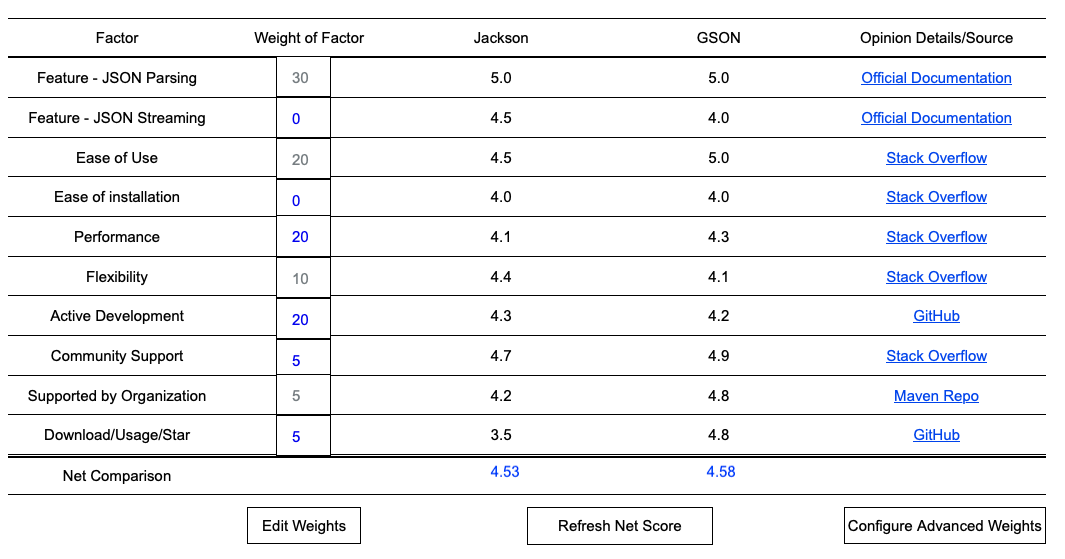
\includegraphics[scale=0.4]{images/mock-ui-library-comparison-2.png}
    \caption{Mock up of a sample comparative analysis of two libraries.
    Some default weights can be provided at the beginning and developers can be able to update the weights (blue-colored weight means the weight is modified by the developer). The score under each library is provided for each aspect and should be ideally calculated by mining the source shown in the Opinion Details/Source column.}
    \label{fig:ui-library-comparison}
\end{figure*}

The first column in the comparison chart contains a few decision-making functional and technical factors. The second column Weight of Factors takes input weights from the developers for their particular situation. The scores under two libraries' columns (Jackson and Gson) contain an aggregated score from the data analysis on respective factors. For example, to measure the score of ease of use, we would mine developers' sentiment in Stack Overflow regarding the specific libraries and come up with a score out of five based on the positive or negative comments shared there. Some scores can be populated using quantitative data collection such as extracting Star (favorite) or measuring recent development activity from GitHub. We would also share the reference of the actual sources from which we are measuring this score in the last column Opinion Details/Source. The final outcome of the analysis is the net comparison of the weighted average score calculated using the Multiattribute Model equation \ref{eq:multiattribute-model}, referred to earlier for each of the two libraries shown in the bottom summary line in blue color. 



\subsubsection{Evaluation of the Library Selection Tool}
All the interviewees highly appreciated such a structured approach to a highly subjective decision that they need to take on a regular basis. Interviewees found the side-by-side numerical comparison to be helpful and suggested a few improvements. For example, instead of providing numerical weight factors, some of them suggested keeping the weights in the backend and in the interface just letting the user choose and rank up and down the priority of the aspects. Some of them also asked for the possibility of manual curation to add new libraries or relevant comments. Most of them requested some way for drilling down to see how the scores are created with some actual references:
\qi{I think that the idea of comparing libraries is quite interesting. If I can click into the underlying sources, then that's pretty interesting for me. I would really value somehow seeing some samples.
... It might be interesting as well to consider whether there is a way to combine both the automated approach plus curated one. People can easily add if there is another library they think should be added.}{P18}

The weighted average decision-making process that was inspired by Fishbein Multiattribute Model \cite{fishbein1967attitude} from the consumer model resonated with most of the participants:
\qi{Yeah. I really like the concept and I'm glad you showed this as an example because I myself have done these sorts of comparisons between Gson and Jackson multiple times. And I really like the variable weight feature because that makes sure that you can focus on what is important for your use case.}{P13}

We assume that future research work can implement the large-scale online review mining and summarize the performance of libraries following this proposed comparative analysis to provide a helpful tool to the developers.

\subsection{Library Selection using ChatGPT and BARD}
\subsubsection{Motivation for Using ChatGPT and BARD}
We conducted the majority of our interviews during the second half of 2022 and a few interviewees mentioned about the usage of ChatGPT\footnote{\url{https://openai.com/blog/chatgpt}} for library-related information collection sources. However, during the analysis part in the first half of 2023, ChatGPT became the fastest-growing consumer application in history \footnote{\url{https://www.reuters.com/technology/chatgpt-sets-record-fastest-growing-user-base-analyst-note-2023-02-01/}}. In February 2023, Google also released similar generative AI-based conversational chatbot BARD \footnote{\url{https://blog.google/technology/ai/bard-google-ai-search-updates/}}. 
If these chatbots can reliably provide library comparison, then this could be a significant support for developers. 
Hence, for the sake of the completeness of study, we wanted to assess the potential usage of ChatGPT and BARD in the library selection process. 

\subsubsection{Experiment with ChatGPT and BARD for Library Selection}
To generate a similar comparison of our proposed mock UI, we provided the following prompt to both ChatGPT and BARD: 
\begin{quote}
  \textit{  Compare Jackson and GSON libraries based on the following aspects (JSON Parsing, Ease of use, Performance, Flexibility, Active Development, Community Support, Supported by Org, Download) in a comparison table. Rate each aspect out of 5 for each library.} 
\end{quote}
Both chatbots provided a tabular comparison against the above prompt as shown in Figure \ref{fig:chatbot-comparison}
\begin{figure*}
    \centering
    \begin{subfigure}{.48\textwidth}
    \centering
        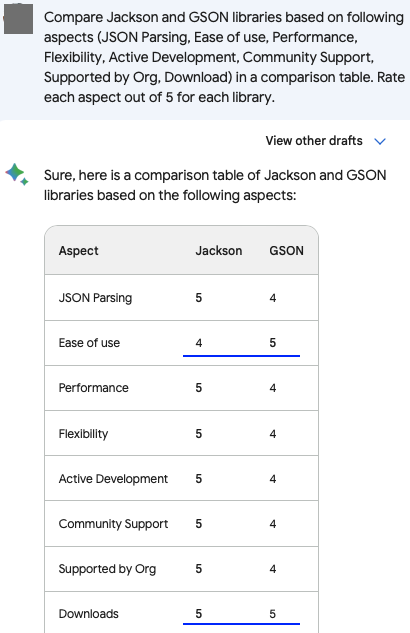
\includegraphics[scale=.5]{images/BARD-Response.png}
        \caption{Response from BARD}
    \label{fig:bard-table}
    \end{subfigure}
    \begin{subfigure}{.48\textwidth}
    \centering
        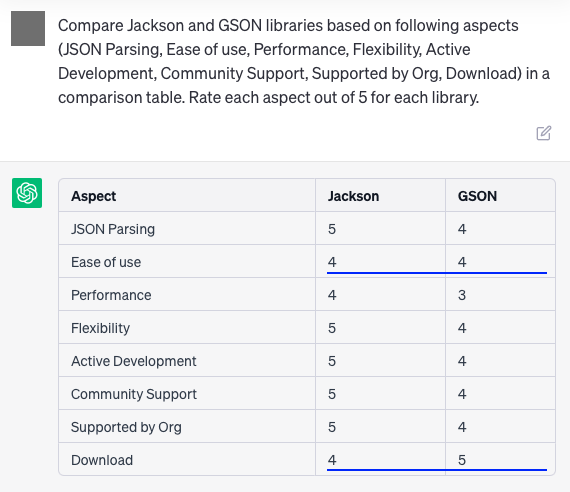
\includegraphics[scale=.4]{images/ChatGPT-Response.png}
        \caption{Response from ChatGPT}
    \label{fig:chatgpt-table}
    \end{subfigure}
    \caption{Response of BARD and ChatGPT for comparing two libraries along with scores.}
    \label{fig:chatbot-comparison}
\end{figure*}

Apparently, both of the models preferred Jackson over GSON. The response shows inconsistent scores between the two models for two different aspects - \code{ease of use} and \code{download count} (\code{download count} is used as an indicator of \code{popularity} factor). BARD gave Jackson (4) a lower score than GSON (5) for \code{ease of use} whereas ChatGPT scored both the same (4). ChatGPT gave Jackson (4) a lower score than GSON (5) for \code{download count} whereas Jackson scored both same (5). Other than these two contradictions, seemingly the chatbot responses were reasonable. Still, we wanted to check the reliability of the response using another small test.

Since in order to identify the score of \code{ease of use} for the two libraries, we shall have to collect reviews online or from other practitioners, we rather chose the \code{download count} which can have a more objective data point. We then asked both chatbots the following prompt: \textit{What is the artifact usage count of Jackson and GSON libraries?}

ChatGPT could not provide any numeric answer because its cutoff date is before September 2021. So we chose BING chat\footnote{\url{https://www.microsoft.com/en-us/edge/features/bing-chat}} to represent ChatGPT since BING chat also uses the same underlying GPT model as ChatGPT. The response from BING chat and BARD are shown in Figure \ref{fig:chatbot-comparison-download}. As we can see, BARD reported the libraries to be used in more than 1.2 million artifacts whereas BING chat referred to an online article and reported that these libraries are downloaded only 14 times (GSON) and 1 time (Jackson). In really, we checked the Maven central repository and found that both of the libraries are used in around 20 thousands of artifacts\footnote{\url{https://mvnrepository.com/artifact/com.fasterxml.jackson.core/jackson-databind/usages}}$^,$\footnote{\url{https://mvnrepository.com/artifact/com.google.code.gson/gson/usages}}.


\begin{figure*}
    \centering
    \begin{subfigure}{.48\textwidth}
    \centering
        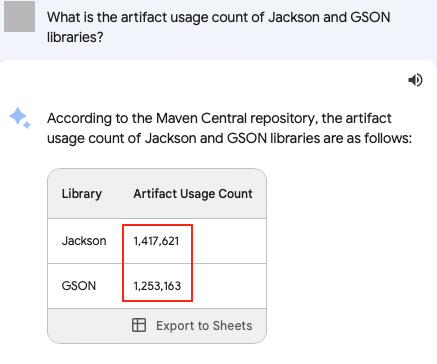
\includegraphics[scale=.45]{images/BARD-donwload-count-1.png}
        \caption{Response from BARD}
    \label{fig:bard-download}
    \end{subfigure}
    \begin{subfigure}{.48\textwidth}
    \centering
        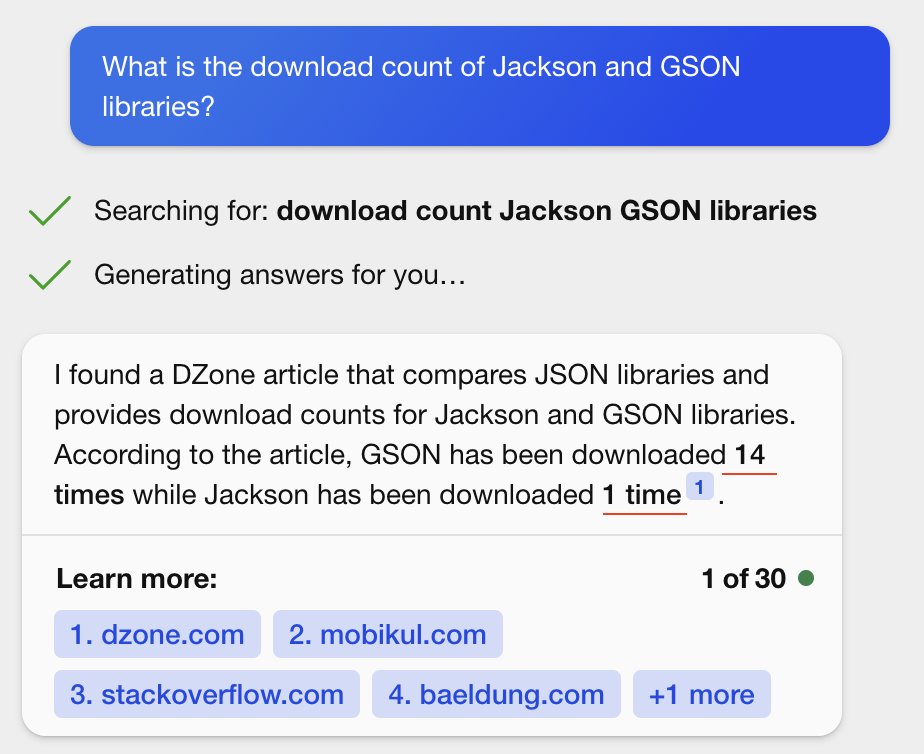
\includegraphics[scale=.45]{images/BING-download-count.png}
        \caption{Response from BING Chat}
    \label{fig:chatgpt-download}
    \end{subfigure}
    \caption{Stark contrast in response from BARD and ChatGPT for the usage count of Jackson and GSON libraries. According to BARD, both of these libraries have been used for more than 1 million times and according to BING chat these libraries are downloaded less than 100 times.}
    \label{fig:chatbot-comparison-download}
\end{figure*}

The small experiments raised concern about the reliability of the responses of the chatbots for the library comparison analysis. We were then curious if the industry practitioners also find similar reliability concerns and how they are considering using chatbots for the library selection process.


\subsubsection{Evaluation on the Usage of ChatGPT and BARD for Library Selection}
We conducted a survey to collect insights regarding chatbot usage among the interviewees. 20 out of 24 interviewees responded to our anonymous online survey.

\textbf{Survey Settings.} In the survey, we asked whether the practitioners already considered using ChatGPT/BARD and what advantages and disadvantages they consider for using those. Since BARD is available only in limited countries, we created the prompt and response example using only ChatGPT so that respondents can recognize familiar tools easily. Also, since we already experimented with Jackson and GSON libraries, we queried about libraries from a different domain (natural language processing - NLP) in the survey.

We asked the following questions in the survey while providing the ChatGPT screenshots when applicable:
\begin{enumerate}
    \item \textbf{Reliability on ChatGPT Response.} We asked participants how much they would rely on the response of ChatGPT against the prompt \textit{"What is a good library in Python for NLP?"}.
    \item \textbf{Next Action after ChatGPT Response.} We then asked an explanatory prompt to ChatGPT \textit{"How easy it is to use Spacy?"}, and asked the participants what would be their next action plan - whether they will trust the response to install the library instantly or will further inquire inside or outside ChatGPT.
    \item \textbf{Comparing Data Interpretation between ChatGPT and Human.} Since ChatGPT is based on a language sequence model that can predict the next token and is trained on undisclosed online data, it was interesting to see how it responds when we give specific library reviews extracted from Stack Overflow. So, with a given review data, we prompted ChatGPT \textit{"How easy it is to use the library strictly based on the given conversation?"}. Then we asked the survey participant whether they agree with the response ChatGPT provided or not.
\end{enumerate}
After the above specific ChatGPT scenarios, we asked the participants their opinion about the quality and reliability concerns of ChatGPT along with their recommendations for future improvement.

\textbf{Survey Findings.}
\begin{enumerate}
    \item \textbf{Usage of ChatGPT.} 
    50\% of respondents said they did not consider using ChatGPT for library selection. The primary reasons they did not consider ChatGPT were lack of reliable research on ChatGPT response, lack of reference for the response, and lack of credibility of the response: \quotebox{}{I have not started using it yet. Chatbots like ChatGPT summarize the comparisons quite well. But they do not always include references and hence credibility needs to be cross-checked almost always.}
    Only 15\% responded that they started using ChatGPT. They considered ChatGPT as an initial high-level information source and they also shared the quality concerns: \quotebox{}{Yes, I have considered chatbots to select and compare libraries. It gives me an initial idea about different libraries quickly without checking search engine results.}
    The rest of the participants did not explicitly mention whether they are using it or not. 
    \item \textbf{Reliability on ChatGPT Response.} 
    No participant said that they would fully rely on the response.
    60\% participants considered asking ChatGPT further about the recommended library and 35\% considered asking about alternative libraries.
    20\% participants would not even trust this recommendation as the source of ChatGPT's response was unknown.
    \item \textbf{Next Action after ChatGPT Response.} 
    85\% participants preferred searching online (using search engines) about spaCy (the library that ChatGPT suggested for NLP) and its alternative libraries listed by ChatGPT.
    60\% responded that they would go to the official documentation of the library after the initial ChatGPT response 
    55\% participants would go online and search Stack Overflow or similar sites to learn about other developers' opinions.
    55\% participants would choose to ask ChatGPT again to provide API samples. 25\% would have doubt about the opinion of ChatGPT and would ask it further elaborative questions.
    
    \item \textbf{Comparing Data Interpretation between ChatGPT and Human.}
    We got mixed results from participants on whether they agreed with the ChatGPT response when a specific library-related conversation was provided. 50\% respondents disagreed with ChatGPT's answer, 20\% agreed and the remaining 30\% were not sure about the correctness of the response provided by ChatGPT.

    \item \textbf{Recommendations for Library Selection}
    The majority of the respondents (85\%) suggested providing additional references to online data sources to support the response of ChatGPT. 20\% participants opined that further challenging questions could be asked to ChatGPT. Some of them also recommended developing a domain-specific chatbot tuned specifically for reusable libraries that can provide better answers compared to general-purpose chatbots.
\end{enumerate}

 In general, the majority of participants shared strong opinions against the reliability, consistency, and validity of ChatGPT responses. They could consider it as an initial discovery source but would not make the final decision based on it. One participant summed it this way: 
 %\ab{Quote this the same way you quote interviews}
 \quotebox{}{I never trust anything chatbot returns, but it's still helpful for research. It's helpful to treat it as the smart, loud, slightly drunk guy at the party. You may gain some great info, but you really don't trust anything he says.}

 
\subsection{Tool Agnostic Relative Priorities of Library Selection Factors}
Because of the reliability concerns of ChatGPT and BARD in library comparison tasks, future researchers might need to develop some comparison tools based on large-scale data mining techniques to calculate the aspect-specific scores as outlined in section \ref{sec:mock-up} or will need to refine the response of those chatbots. However, we found from the industry evaluation that practitioners would always need to use variable priorities depending on their conditions. Interviewees also suggested providing some default priorities to help developers update according to their needs. Hence,
it would be a great convenience if we can provide a default factor-wise priority or weight score in the comparison tool.

%During our interviews while we discussed about library selection factors, we often asked developers whether they treat all the factors equally important. All participants unanimously expressed that all the factors have different priorities to them in general. That was also one motivation to provide weight of the factors in the comparison tool described in previous section. Though we explained in detail that guiding principles influence the library selection factors to great deal, we realized that a generic priority of library selection criteria would be helpful for developers' common understanding and for implementation of any comparative analysis tool.

% Table generated by Excel2LaTeX from sheet 'Priority of factors'
\begin{table}[htbp]
  \centering
  \caption{Relative priorities of library selection factors. The higher score reflects higher priority practitioners put on when selecting a third party library. The priority score is normalized out of 10. Our recommended cut-off factors are marked with asterisk (*).}
    \begin{tabular}{llr}
    \toprule
    \textbf{Factor} & \textbf{Category} & \multicolumn{1}{l}{\textbf{Priority}} \\
    \midrule
    Performance & Software &                 8.2  \\
    Stability & Software &                 7.8  \\
    Licence* & Commercial &                 7.5  \\
    Documentation & Commercial &                 7.3  \\
    Security* & Software &                 6.9  \\
    Compatibility* & Software &                 6.4  \\
    Active Development & Maintenance &                 6.2  \\
    Popularity & External &                 6.0  \\
    Supported by Own Organization & Maintenance &                 5.9  \\
    Ease of Use & Software &                 5.5  \\
    Capability of Library* & Software &                 5.5  \\
    Dependency & Commercial &                 5.4  \\
    Flexibility & Software &                 5.4  \\
    Open Source Software & Commercial &                 5.2  \\
    Community Support & Maintenance &                 5.2  \\
    Cost  & Commercial &                 5.1  \\
    Used by Reputed Companies & Maintenance &                 4.9  \\
    Availability of Demo & Commercial &                 4.8  \\
    Large Community & Maintenance &                 4.5  \\
    Supported by Reputed Organization & Maintenance &                 4.4  \\
    Customer Support & Maintenance &                 4.4  \\
    Familiarity & External &                 4.3  \\
    Size of Library & Software &                 4.2  \\
    Search Engine Ranking & External &                 4.1  \\
    Ease of Installation & Software &                 3.6  \\
    Interesting Interface & Software &                 2.7  \\
    Detailed Benchmark & External &                 2.6  \\
    Roadmap & Commercial &                 2.4  \\
    \bottomrule
    \end{tabular}%
  \label{tab:factor-priority}%
\end{table}%

In this regard, during the member checking survey (described in the quality evaluation section), we also asked our interview participants how they compare among all the 28 library selection factors. For each factor, we let them choose a score on a sliding scale of 20. We used the ``Statement randomization'' feature of Qualtrics\footnote{\url{https://www.qualtrics.com}} software to randomize the list of the selection factors to avoid response order bias \cite{israel1990can}.

%\ab{Why do you have these blue?}
\td{11} out of \td{13} respondents of the survey provided their scoring of relative priorities of library selection criteria. Table \ref{tab:factor-priority} shows the average priority of selection factors normalized on a scale of 10. Participants chose \code{performance}, \code{stability}, \code{license}, \code{documentation}, and \code{security} as their top priority factors. Though we observed that the {\principle} can significantly influence the priority of these factors, we recommend \code{security} and \code{license} to be `cut-off' factors for any team so that they do not compromise with non-supported license and security vulnerabilities. We observed that two other factors \code{capability of library} and \code{compatibility} are also cut-off factors in the sense that if a library is not compatible with the target environment and does not perform the intended task, there is no point in using such a library. We marked these four factors with an asterisk to denote them as cut-off factors in Table \ref{tab:factor-priority}. We believe any future research could enhance this generic priority of factors to a more customized priority score followed by the {\principle} to respect the conditions of particular organizations and development teams.
\section{Discussion} 

\subsection{Recommendations}

We have observed that even before being able to integrate a library, there are certain \code{conditions}  of an organization or a developer which may prevent them from considering a library at all. Obstacles can be caused by organizational policy, technology, or even by the developer's mindset and experience. In some cases, a lack of supportive processes, such as an Open-Source Software Office (OSPO), or restricted internet access meant that developers lacked clarity about which libraries could be used. 
\begin{recommendation}{rec:ospo}
  {Organizations should formalize 
third-party library policy, and create streamlined processes to support it.}
\end{recommendation}\medskip

For developers and organizations the use of libraries not only brings benefits, it also brings disadvantages which must be considered. Participants noted that often developers can focus on solving imminent problems in hand and have a blind spot on the future maintenance of a library. However, as we have observed, library maintenance is a major part of the adoption process and developers should be aware of the \code{post integration maintenance} period. 
\begin{recommendation}{rec:maintenance}
  {Organizations should have a library maintenance strategy for upgrading libraries and consider it during selection.}
  %{Organizations should have a strategy for maintaining and upgrading libraries, which is also considered during the library selection process.}
  %Developers not only need to consider the maintenance related concerns while reviewing a library, they also need to deploy a strategy to continually maintain or upgrade libraries. The strategy may involve developing organizational policy, or even allocating certain resources for future maintenance.}
\end{recommendation}\medskip

Though we presented the conditions of each guiding principle separately, in reality, developers may have multiple types of conditions with conflicting guiding principles. For example, in a mature organization with large-scale application, a team may face an urgent production issue in a critical feature that may prompt \code{Just Do It} principle immediately, however, they will need to adopt \code{Reuse Robust Component} once the urgency diminishes. %The long-term maintainability of a library is not always a consideration in all situations. While it is critical in the guiding principle (GP) ``Ensure Compliance,'' it is of little interest under the conditions where ``Just Do It'' is applicable. 
\begin{recommendation}{rec:gp}
%Developers should identify the appropriate guiding principle or principles before they can begin the library adoption steps.
Developers should consider multiple {\principle} when faced with complicated and conflicting conditions. 
\end{recommendation}\medskip

Marketing theories consider cut-off factors as those factors of the product whose absence will bar the consumer from buying it \cite{blackwell2001consumer}. 
% \\% AB: This is a horrible hack to force line fitting.
During our interviews, participants observed that all developers consider \code{capability} and \code{compatibility} of libraries as such cut-off factors. However, they also noted that developers in a few conditions (\code{small} or \code{early stage} organizations, or \code{early career} developers) may be unaware of the severity of security and license issues and may ignore those. Industry experts strongly recommended  considering compliance issues as cut-off factors.
 \begin{recommendation}{rec:cutoff}
Organizations should consider \code{security} and \code{license} issues, irrespective of \code{organizational} or \code{environmental} conditions.
\end{recommendation}\medskip
Developers seek information from a variety of sources. If the organization does not have a very welcoming, inclusive culture, critical analysis of libraries can be ultimately influenced and driven by outspoken people. We have heard from the interviewees about the necessity of inclusive culture where they assumed that inclusivity should prevail in a software development team from the beginning of the recruitment process up to the development team's regular discussion. However, it was also evident that even in larger well-managed organizations, such inclusivity may remain very subtle and may not be able to promote a democratic decision throughout the library selection process. It would be the responsibility of the team leader to let normally silent members communicate their ideas in whatever preferred (verbal, written) way possible.
 \begin{recommendation}{rec:inclusivity}
Organizations should encourage openness and inclusivity to support developers' diverse communication styles. 
\end{recommendation}\medskip
 Even when the culture promotes openness, development teams often have few enthusiastic developers who love to explore and whose opinions might have a disproportionate weight in discussions. Teams are better when all members will develop a habit of regular studies and in the long run, they will be able to adapt much better to technological changes as well as make decisions about third-party tools or libraries in general. We found from the participants that enthusiastic early career developers often care about getting things done and frequently want to try out new libraries for the richness of their careers (or resume). %However, raising the concern of the lifelong maintenance of third-party libraries, interviewees recommended to avoid libraries when it is not necessary. 
 Providing sanctioned, scheduled opportunities for learning allow experimentation with new technologies without jeopardizing the production system.
  \begin{recommendation}{rec:hackathon}
  Organizations should promote a culture of technical exploration and discussion through study circles or hackathons.
% To promote the culture of technical exploration and discussion, a team can decide to go for weekly studies and form a study circle where every developer will present something new that they learnt, or implement yearly hackathons where developers can experiment with new technologies without jeopardising the production system. 
\end{recommendation}

There still is a lack of guiding tools that can support library selection (or in general, technology selection) by summarizing a large amount of data according to the team's priorities. Developers cannot rely on the existing summarization research outcomes since the detailed reference and quality assurance of those tools still are not considered worthy of industrial usage.
  \begin{recommendation}{rec:summary-tool}
  Researchers and tool developers can consider developing reliable library selection tools that can properly mine the online reviews and also provide the references of the summaries.
\end{recommendation}

\subsection{Implications}
Our research presents the software library adoption model for the first time, along with a detailed description of conditions, factors, and patterns affecting the selection process. Unlike earlier work, which found 26 human and technical factors associated with adoption \cite{larios2020selecting}, we divide aspects of the selection process into different categories and identified 14 new conditions. 
We also present six \principle, which can be readily recognized by the industry. 
We supplement these with recommendations drawn from the interviews on how the industry can more effectively prepare for and use third-party libraries. 

% \begin{figure}
%     \centering
%     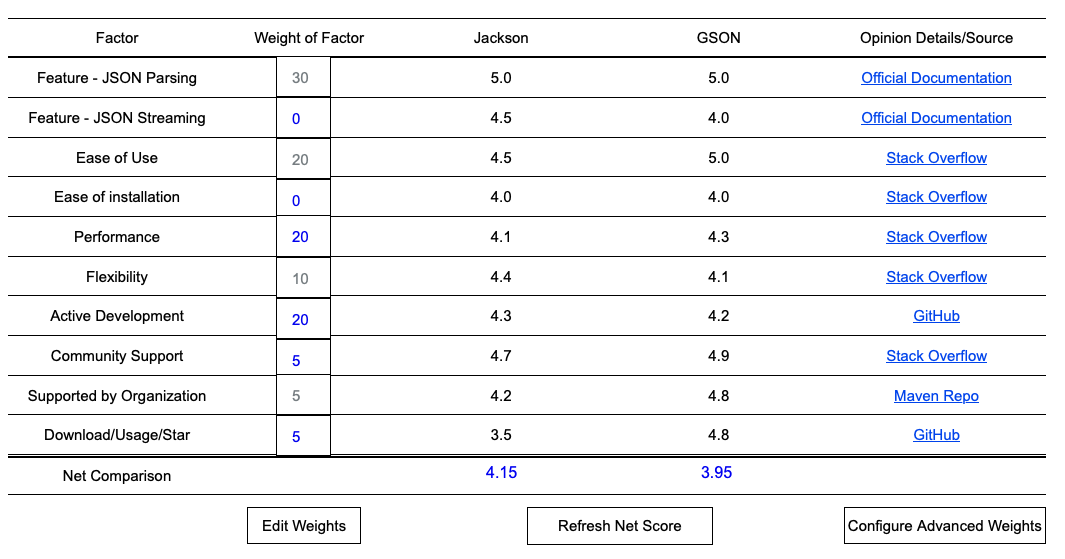
\includegraphics[scale=.25]{images/mock-ui-library-comparison.png}
%     \caption{A mock-up user interface for comparing multiple libraries along with weight of each library specific factors}
%     \label{fig:mock-ui-library-comparison}
% \end{figure}
The interviews also informed us of the feasibility of creating a tool that can help compare software libraries to support their adoption. One of our participants, a consultant with 22 years of experience, was explicit with the needs of such a tool: \qi{Let's say I would like to install a module and I would like to find the third-party library. I would like to have an easy way to see and I approve. I don't see any tools really for that. In many cases, I saw this: a page is trying to compare libraries but there is no objective way to compare them. Maybe there is, but there's not implemented... So that's part of the reason people don't use [libraries] because they say, OK, I don't know which one to use. This is a general problem.}{P22}

In our later interviews, we presented developers with a mock-up of such a tool, the development of which is our ongoing research. The tool design was influenced by the Fishbein Multiattribute Model \cite{fishbein1967attitude}, which aims to facilitate consumer purchase decisions by assigning weights to different factors of a given product and then using the weighted averages across products to rank those. In our tool mock-up UI, we thus suggested to simply assigning weights to each factor (e.g., \code{performance}) of a software library. The weights would be collected from representative sources (e.g., based on user reviews on the \code{performance} aspect of a library) and from a developer (e.g., the relative importance of a factor like \code{performance} over another factor like \code{usability}).
The participants who reviewed the tool during the interview also appreciated such an approach: 
%\qi{It would be a really great tool to select some libraries because it's like our processes, we choose a library because of our own subjective or objective factors and here you have the right factors. So you can build our process with your tool. I think we can use it in our company.}{P17} % [MINAOAR] Revised this quotation for making spacr for Data Availability.
\qi{It would be a really great tool to select some libraries because it's like our processes, we select first some keywords and afterward, we choose a library because of our own, sometimes subjective, sometimes objective factors and here you have the right factors so you can build our process with your tool. I think we can use it in our company.}{P17}

We also analyzed the feasibility of using large language model-based chatbots (BARD and ChatGPT) for the library selection process. However, the industrial evaluation survey reflects that such chatbot responses further need to be verified and supplemented with other reliable online references. Their detailed feedback can support future researchers or developers designing chatbot-based library selection tools.

%The Fishbein Multiattribute Model \cite{fishbein1967attitude} can be extended to theorize library selection process through the use of marketing lens. 



% (e.g., \code{company}, \code{application domain}, \code{investment capacity}) and 15 additional selection factors (e.g., \code{ease of installation}, \code{flexibility}, \code{availability of demo}, \code{familiarity}). 
% We were further able to identify eight novel information sources such as \code{known people}, \code{search engine}, \code{existing source code}) compared with an earlier study on collecting information about open source software \cite{li2022exploring}. 

%As part of the adoption process, we have presented 5 major steps of library adoption process, identified 28 library selection factors, 14 library related source of information, and 23 internal external conditions that influence the process. No other previous study provided the process steps for libraries. Larios-Vargas et. \cite{larios2020selecting} identified 26 factors influence library selection under technical, human resource, and economical factors. Their proposed human resource and economical factors are fully mapped by our conditions category and technical factors are covered by our library selection factors. We identified 14 new conditions (such as \code{company}, \code{application domain}, \code{investment capacity}, \code{Expert/lead opinion}, \code{upgrades of OS}, \code{criticality of feature}, \code{delivery deadline}) beyond their human and economic factors. Moreover, our study also found 15 additional software selection factors (such as \code{ease of installation}, \code{flexibility}, \code{availability of demo}, \code{familiarity}, \code{used by reputed company}) which their study did not report. Besides, the factors, Li et. al outlined 14 sources for collecting information about open source software (not library) \cite{li2022exploring}. All of their reported sources are covered by our 6 information sources (\code{Package repository}, \code{Source repository}, \code{Stack Overflow}, \code{Other Q\&A sites}, \code{Online Article}, \code{Influential Blog}) and 8 of our sources are novel (such as \code{known people}, \code{search engine}, \code{existing source code}) for library information.}


\section{Quality and Applicability of the Study}
In our study, in the first part, we developed a library selection model following grounded theory methodology, and in the second part, we conceptualized and evaluated two different library selection tools based on the library selection model. Since the library selection tools are already evaluated by the industrial survey, the grounded theory-based model preparation part of the study remains subject to further evaluation. In this section, we evaluate the quality and applicability of our grounded theory research for the development of the library adoption model.

Corbin and Strauss did not recommend using the terms `validity' and `reliability' when discussing qualitative study \cite{corbin2014gt}, because qualitative methodologies cannot be assessed using quantitative criteria. They defined 17 measures researchers can use to evaluate the quality and applicability of their grounded theory research. We present the complete evaluation as part of our replication package \cite{website:replication-package}, here we present five major evaluation criteria.

\subsection{Industry Fitness}
This criterion concerns industry credibility. We conducted member checking \cite{creswell2016qualitative} by presenting a ten-page summary of our findings, which was sent to 18 of our interviewees who agreed to further contact. This communication included a link to a survey that asked their opinion as to whether the summary reflected their experience and was useful to them. Thirteen participants completed the survey, all of whom opined that the summary was accurate. Five provided detailed feedback on the findings:
\qi{I think the summary captures different aspects of the library selection process very well. It outlines a generic, industry-wide pattern with enough details, and also provides exceptional factors that impact that pattern.}{}

\subsection{Industrial Application} Industrial application answers the question of whether the findings provide insight into situations and provide knowledge that can be applied to develop policy, change practice, and add to the knowledge base of a profession \cite{corbin2014gt}. %This criterion was also evaluated through member checking.  %[MINAOAR] commented this line for Data Availability space.
In member checking, one participant shared their feedback, demonstrating that they found our work applicable: \qi{One interesting thing that I learned from your research is, different developers have different processes and priorities for picking a library, and not everybody is considering all the steps that need to be taken, so I would recommend your paper to all developers to just widen their horizons.}{}

\subsection{Usefulness} To address this measure, we looked at if there are suggestions for practice, policy, teaching, and application \cite{corbin2014gt}. %To the best of our knowledge, this is the first study to provide a comprehensive picture of library adoption. %[MINAOAR] commented this line for Data Availability space.
The presentation of guiding principles in the form of patterns, which are widely used in industry, makes the results more accessible to practitioners. Participants also appreciated the suggestions:
\qi{My favorite part of the summary is the takeaway action items that I believe would be useful in building a better culture for adopting the right tools and technologies.}{}

\subsection{Explainability of Theory} The way to assess this measure is to determine if variation is built into the theory \cite{corbin2014gt}. Our conceptual framework is based on six {\principle} which depend on different contexts and lead to different implications for the influence of conditions, factors, and use of information sources. This allows the theory to support a wide variety of circumstances.

\subsection{Saturation of Categories} ``How is saturation explained, and when and how was it determined that categories were saturated?'' is the criterion for evaluating this measure \cite{corbin2014gt}. We provided detailed information about how we performed theoretical sampling to achieve saturation and described how the major categories achieved saturation throughout the progression of the study. Figure \ref{fig:saturation} contains a heatmap of concept saturation which shows the progression of topics across interviews.

\subsection{Threats to Validity}
\bf{Construct validity} threats concern the relation between theory
and observations. In our study, they could arise if there is a lack of accuracy in the open coding. To mitigate this threat, two of the authors conducted the coding of several interviews separately and then discussed their codebooks with each other. This approach helped us mitigate the presence of subjective bias in the coding. Threats to \bf{external validity} compromise the confidence in
stating whether the study results are applicable to other
groups. Our library adoption model is derived from the semi-structured interviews of 24 professional developers from multiple international large and small-scale software companies. We carefully adopted a theoretical sampling approach to recruit our study participants, which ensured that we collected as diverse opinions on library adoption as possible. Future studies could extend our study findings with more interviews or surveys, however, we expect that the core findings will remain.




\section{Conclusion}
Software library adoption includes the selection as well as the maintenance of a library. In this paper, we conducted \numInterviews semi-structured interviews to explore the major steps developers follow in the adoption of a software library. We present a novel library adoption model that consists of the process that developers follow to adopt a library, and a set of conditions, information sources, factors, \principle\space that influence the process and barriers that developers face. We conceptualized a useful library selection tool and evaluated the usage of ChatGPT/BARD for library selection.
We proposed seven recommendations derived from the concerns that developers identified in interviews. Our study provides researchers with the opportunity to investigate specific adoption steps in more detail. The factors can be used to develop comparative analysis tools. Additionally, the industry can make use of the existing patterns and recommendations to guide decisions about third-party library selection. Our future work focuses on the development of a toolkit to support the automatic comparison of software libraries based on our derived library adoption model.
% As part of the adoption process, we presented five steps of the process, with 18 associated concepts. We showed how five conditions, consisting of 23 concepts, influence the choice of guiding principle, which in turn influences the weight of factors and the sources of information used to inform the adoption process. The four factors contain 28 concepts, while the five categories of information sources have 14 concepts associated with them.

\section{Data Availability}
% [MINAOAR] I have removed two senteces and revised one quotation in Discussion section for making space for Data Availability section. Those changes are tagged with [MINAOAR].
Codebook, study evaluation and interview script (no interview transcription is available based on the approved research ethics application) are available at \cite{website:replication-package}.
%Our replication package contains the interview script, invitation emails, consent form, final codebook, assessment of grounded theory evaluation criteria, and an Appendix \cite{website:replication-package}. In order to adhere to our ethics approval, we do not share a list of interview participants or the interview transcripts. 


% The conceptual framework of adoption process should provide the researchers the opportunity to investigate more into specific adoption steps. The factors can be used for developing comparative analysis tools for libraries. Researchers in the techno-social community can study the individual and organizational conditions that interplay in the library adoption process.

 
% The other major contribution of our research is the guiding principles. These principles not only explain the influences and activities in library adoption process, but also provide a concrete guideline for developers working in complex conditions to adopt libraries appropriately.




%\input{F.challenges}



%%
%% The acknowledgments section is defined using the "acks" environment
%% (and NOT an unnumbered section). This ensures the proper
%% identification of the section in the article metadata, and the
%% consistent spelling of the heading.
% \begin{acks}
% \end{acks}

%%
%% The next two lines define the bibliography style to be used, and
%% the bibliography file.

\bibliographystyle{ACM-Reference-Format}
\bibliography{references}
%%
%% If your work has an appendix, this is the place to put it.
%\appendix
%%%%%%%% Appendix
\pagebreak
\section{Methodology}

Figure~\ref{fig:methodology} provides an overview of the overall research method which was applied to the study.

\begin{figure*}
    \centering
    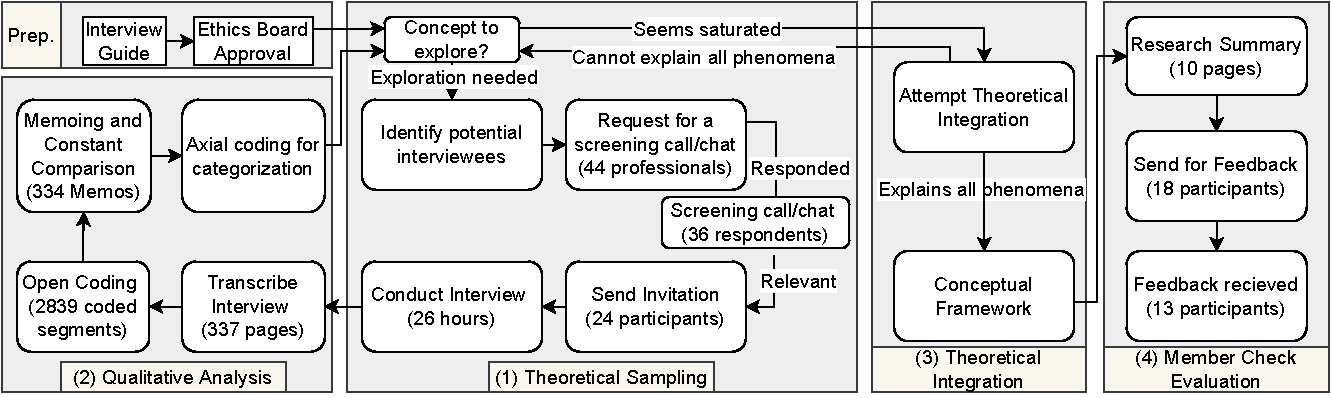
\includegraphics[scale=.75]{images/methodology.pdf}
    \caption{Grounded theory research method applied}
    \label{fig:methodology}
\end{figure*}


\section{Saturation}
\begin{figure*}
    \centering
    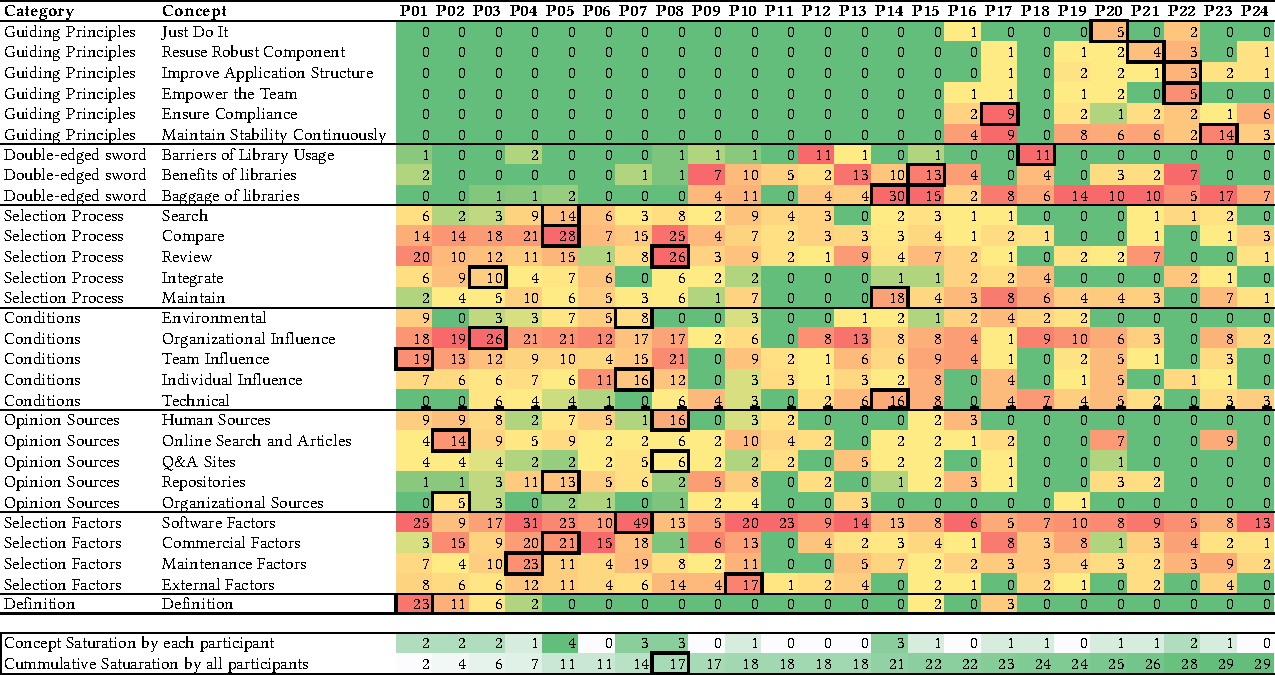
\includegraphics[scale=0.8]{images/saturation.pdf}
    \caption{Heatmap of concept saturation over the interviews. Red refers to higher discussion of a concept by an interviewee, the number refers to how many times interviewee has discussed a concept. Green refers to lower discussion of concepts by an interviewee.}
    \label{fig:saturation}
\end{figure*}
Figure~\ref{fig:saturation} shows how the concepts were discussed during each interview. The number denote how many times a concept was discussed by one particular interview. The more a participant discussed about a particular concept, the more red the corresponding cell is. For example, library search and analysis process was most discussed by P5 and after their interview, subsequently we did not have much to discuss about the search process.  After P8, the concept almost saturated and we discussed very little about this concept with subsequent interviewees.

\begin{table*}[]
    \centering
    \begin{tabular}{p{.4cm}p{4cm}p{6cm}p{6cm}}%{llll}
    \toprule
    P\# & Concept we wanted to enhance & Why we selected this Participant & Concepts they enriched significantly \\ 
    \midrule
P1 & Initial process and factors & Architect of a large system & Library definition, factors, influences \\ 
P2 & Licensing and Security Issues & Working in a large structured company & License, company technology \\ 
P3 & Mobile development Factors & 12+ years experienced in mobile application & Cost, company tech, comparison  \\ 
P4 & Long term maintenance concerns & Being a CEO, takes decisions considering long term impact & Company application domain, active development of library \\ 
P5 & Decision making processes & Stablishing the processes in a startup team & Information search, company culture \\ 
P6 & Open Source factors & Has experience regarding OSS contribution and research & Open source, Personal motivation \\ 
P7 & Factors for a startup & Being a startup CTO may share different priorities & Flexibility, Ease of Installation, Community Support \\ 
P8 & Performance factors & Working in a cloud company that may requiew high performing libraries & Familiarity, Team Discussion, Library Migration \\ 
P9 & Migration scenarios & Experienced to migrate company tech stack as architect & Legal risks, Lack of Stability, Less prefered than native support \\ 
P10 & Visualization and front end libraries & Working as web developer for over a decade & Customer support, flexibility, existing repository \\ 
P11 & Machine learning libraries & Experienced in machine learning in gradudate research studies and in industry & Talk to people, Performance, Outstanding library selection \\ 
P12* & DevOps Process for Library Security Issues & Consulted dozens of companies in DevOps process establishment & Barriers of library usage, Baggage of libraries \\ 
P13 & Selection process in large organizations for legal and security risks & Has been an architect in a large team for 10+ years & Consent Process, Benefits of libraries, Tech Expert Opinion \\ 
P14 & Library migration scenarios & Experienced in managing mobile apps with large user base in all platforms & Make life easy, Life long maintenance, Migration to other library \\ 
P15 & Organizational process and motivation for libraries & Experienced in organization process since increased dev team from 3 to 300 & Delivery Deadline, Don't Reinvent the wheel, Feature criticality \\ 
P16* & Process of security concerns & Cerified security professional actively developing security products & License issues, Data Transfer Security, Geographic Impact  \\ 
P17 & Security Process & Delivers custom software to customers and maintains SecOps in CI/CD & Post Integration Maintenance for Security \\ 
P18 & C++ libraries in large scale long term products & Leads development of a 30 year old product written in C++ with 2M lines of code & Lifelong Maintenance Burden, Compatibility, Uniform Coding Style \\ 
P19 & Company Culture, Open Source, Concept Saturation & Experienced working in start-up and large organizations who open source libraries & Standard practices in large organizations, Considerations in open source \\ 
P20 & Challenges in mobile application libraries, Concept Saturation & Full career in mobile app development, mostly in iOS which requires more maintenance & Lifelong Maintenance Burden, Abandoned Libraries, Migration \\ 
P21 & Company Culture, Open Source, Concept Saturation & Works full-time in a prominent open core company & Company policies, Guiding Principles \\ 
P22 & Guiding Principles, Open Source & Experienced in persuing large corporation for open source library adoption & Guiding Principles \\ 
P23 & ML libraries & Working in South America in ML domain & ML Library Dependency Issues \\ 
P24 & Company Culture, Industry, ML Libraries & Working in health sector using ML libraries extensively. & ML Library deployment and upgrade issues \\ 

\bottomrule
    \end{tabular}
    \caption{How we recruited interview participants following theoretical sampling for Concept Saturation. (We could not enhance targeted concepts from the *-marked participants (P12, P16), rather enriched other important concepts.)}
    \label{tab:theoritcal-sampling}
\end{table*}

%% Ann: this is just an alternate view of our main figure and I don't think it is useful
%\begin{figure}
%    \centering
%    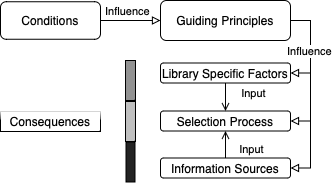
\includegraphics[scale=0.6]{images/Interaction-with-guiding-principles-5.png}
%    \caption{Interaction of guiding principles with the major concepts of software library adoption process}
  %  \label{fig:gp-interaction}
%\end{figure}


\section{Code System}

Figure~\ref{fig:process} shows the relationship between major categories, categories, and concepts in the code system for the major categories steps and source. These concepts and categories contribute to the conceptual framework of the software library adoption process.

\begin{figure*}
    \centering
    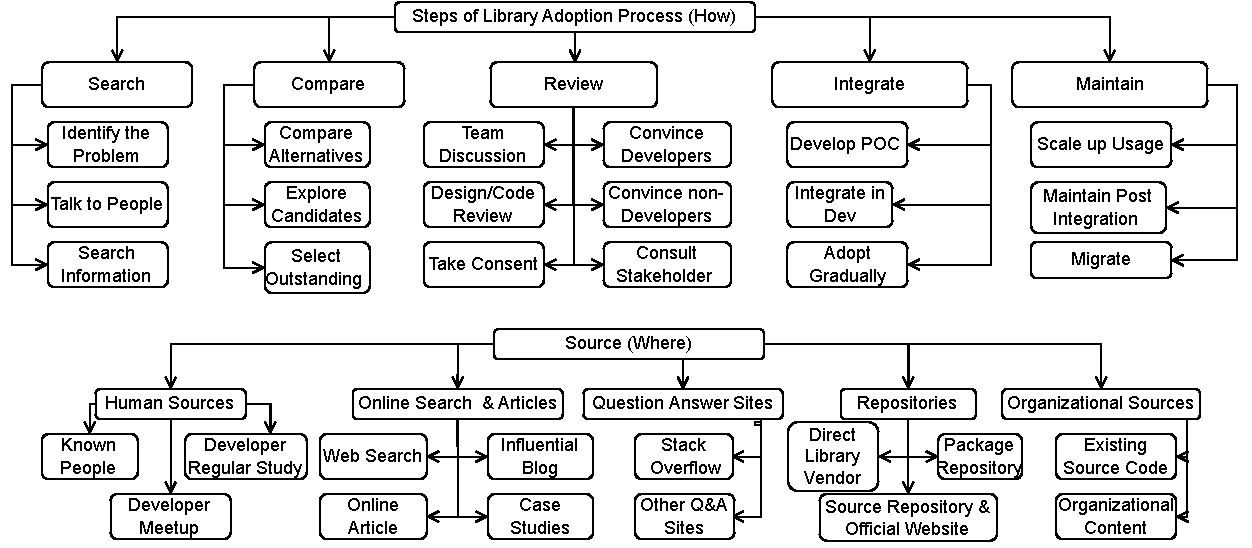
\includegraphics[scale=0.85]{images/process.pdf}
    \caption{Concepts related library adoption process}
    \label{fig:process}
\end{figure*}

%\begin{figure*}
%    \centering
%    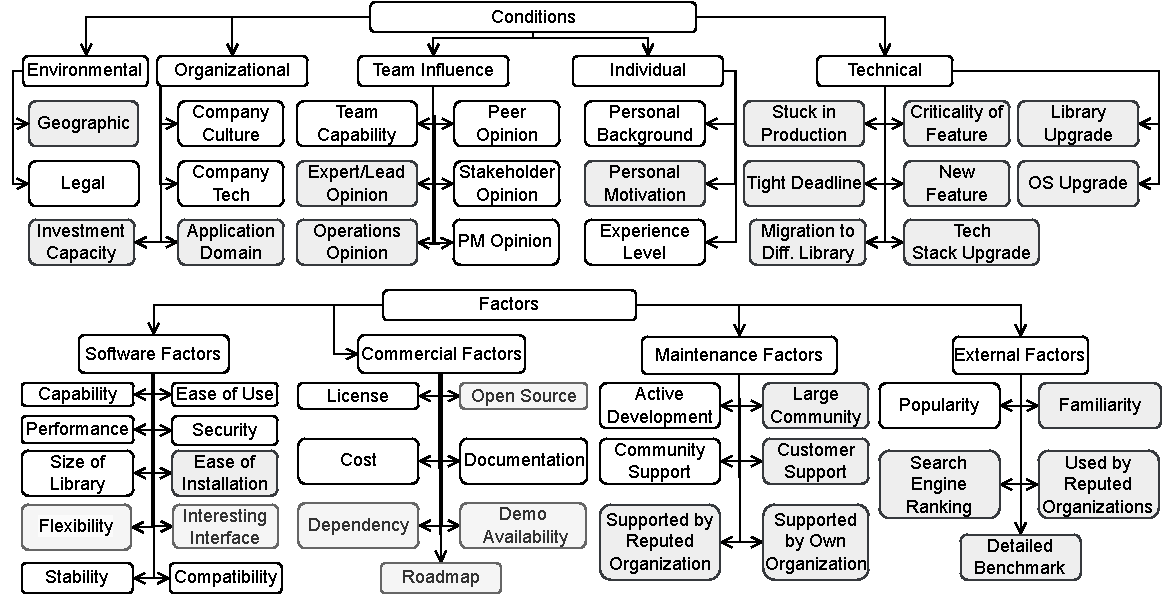
\includegraphics[scale=0.85]{images/conditions.pdf}
%    \caption{Concepts related with factors and conditions %influencing library adoption process}
%    \label{fig:conditions}
%\end{figure*}

\section{Guiding Principles}
In this section, we present the six full patterns associated with the library adoption steps.

\FloatBarrier
\begin{practice}{1}{Just Do It}
\actor{Developers}
\condition{Faster go to market is critical. Developers rewarded for delivering minimum feature on time.}
\concern{How the developers can meet the deadline with relatively less effort?}
\solution{Use a third-party library that reduces the work load and delivery can be done on time}
\consideration{Easy to use, easy to install, popular, and familiar library.}
\steps{Find libraries, compare them, and choose one according to the consideration. Take support from known people or use search engine or Stack Overflow}
\consequence{Can lead to future maintenance burden such as performance bottleneck or security vulnerability.}
\example{For startups, a lot of it [priority] is just speed to market and how much resources is gonna eat up using any specific library.}{P07}
\end{practice}

% \begin{table}[]
%     \centering
%     \caption{Scenario of GP1: Just Do It}
%     \begin{tabular}{p{1cm}p{6.5cm}}
%          \toprule
%             \textbf{GP} & \textbf{Just Do It} \\ 
%             \midrule
%             Actor(s) & Developers \\ 
%             Context & - Faster go to market is critical for business. Developers are often rewarded for delivering minimum viable product on time.
%             - Developers are in their early career and assume higher satisfaction on faster delivery. \\ 
%             Concern & How the developers can meet the deadline in relatively less effort? \\ 
%             Solution & Use a third-party library that reduces the work load and delivery can be done on time \\ 
%             Consider-ation & The library should be easy to use, easy to install, popular, and even better if developer is already familiar with it. \\ 
%             Steps & Find libraries, compare them, and choose one according to the consideration \\ 
%             Support & Take support from known people to know about such library or use search engine, Stack Overflow \\ 
%             Example Trace in Data & For startups, a lot of it [priority] is just speed to market and how much resources is gonna eat up using any specific library. (P07) \\ 
%          \bottomrule
%     \end{tabular}
%     \label{tab:gp1-scenario}
% \end{table}

\begin{practice}{2}{Reuse Robust Component}
\actor{Developers, Senior Developers}
\condition{Mature organization, stable code. Developers concerned of quality, performance \& maintainability.}
\concern{How can the application avoid boiler plate code and follow best design principles?}
\solution{Use a trusted proven third-party library that will keep the code clean and manageable.}
\consideration{Open source, community trusted, stable and high-performing library.}
\steps{Find and compare libraries, review thoroughly by more than one developer. Look into the library's source code repository to analyze the stability, quality of the library, and also consider reputed technical blogs.}
\consequence{Too much analysis and exploration can be an overkill for small features causing delivery delay.}
%\hline
\example{So [this large corporation] as a whole is actually built on the open source libraries that are suitable for our use cases. But that actually has been one of our primary focus as well. If you find a library, use it; only build if you can’t find anything.}{P13}
\end{practice}

% \begin{table}[]
%     \centering
%     \caption{Scenario of GP2: Reuse Robust Component}
%     \begin{tabular}{p{1cm}p{7.5cm}}
%          \toprule
%             \textbf{GP} & \textbf{Reuse Robust Component} \\ 
%             \midrule
%             Actor(s) & Developers, Senior Developers \\ 
%             Context & - Matured organization with stable source code and release pipeline. Application performance and maintainability is a big concern for the team.
%             - Developers with higher experience would be careful about the quality of the application source code. \\ 
%             Concern & How the application can avoid boiler plate code and follow best design principles? \\ 
%             Solution & Use a trusted proven third-party library that will keep the code clean and manageable. \\ 
%             Consider-ation & The library should be open source, trusted by community, stable and provide apppropriate performance metrics required \\ 
%             Steps & Find and compare libraries, review thoroughly by more than one developer. \\ 
%             Support & Look into the library's source code repository to analyze the stability, quality of the library, and also consider reputed technical blogs. \\ 
%             Example Trace in Data & So [this large corporation] as a whole is actually built on the open source libraries that are suitable for our use cases. But that actually has been one of our primary focus as well. If you find a library, use it; only build if you can’t find anything. (P13) \\ 
%          \bottomrule
%     \end{tabular}
%     \label{tab:gp2-scenario}
% \end{table}

%\vspace{-5mm}
\begin{practice}{3}{Maximize Flexibility} % Was Improve Application Structure
\actor{Developers, Architects}
\condition{Large scale software applications have their own structure which evolved over time and may follow some software design principles. System designers want to use new libraries in a way that improves the application structure, or at least does not deteriorate it.}
\concern{How can the architecture be improved or be protected from unwanted rigidity while using a library?}
\solution{Use a library that just fits right with the application in terms of the size and flexibility. Consider wrapping the third-party library in an API to allow replacement of the library without affecting dependent code.}
\consideration{The library should be flexible and should not be too large in size compared to the system.}
\steps{Find, compare, and review libraries. Conduct design review to assess impact on architecture. Review internal organizational content for design principles.}
\example{The moment you have to bring something in because there are new requirements is the time to assess how you've structured your application and does it still serve you and your customers or the business requirements you have. So that’s the opportunity to look at the structural aspect of the application and make sure you do want to avoid changing it or maybe
it's the time to change it.}{P22}
\end{practice}%\vspace{-4mm}

% \begin{table}[h]
%     \centering
%     %\caption{Scenario of GP3: Maximize Flexibility}
%     \begin{tabular}{p{8.5cm}}%{p{1cm}p{7.5cm}}
%          \toprule
%          \textbf{Guiding Principle 3 - Maximize Flexibility} \\% & \textbf{Improve Application Structure} \\ 
%          \midrule
%             \bf{Actor(s).} Developers, Architects \\ %\midrule 
%             \bf{Condition.} Large scale software applications have their own structure which evolved over time and may follow some software design principles. System designers want to use new libraries in a way that improves the application structure, or at least does not deteriorate it.\\ %\midrule 
%             \bf{Concern.} How can the architecture be improved or be protected from unwanted rigidity while using a library?\\ %\midrule 
%             \bf{Solution.} Use a library that just fits right with the application in terms of the size and flexibility. Consider wrapping the third-party library in an API to allow replacement of the library without affecting dependent code.\\ %\midrule 
%             \bf{Consideration}. The library should be flexible and should not be too large in size compared to the system.\\ %\midrule 
%             \bf{Steps.} Find, compare, and review libraries. Conduct design review to assess impact on architecture. Review internal organizational content for design principles.\\ %\midrule 
%             \bf{Example}. \emph{``The moment you have to bring something in because there are new requirements is the time to assess how you've structured your application and does it still serve you and your customers or the business requirements you have. So that’s the opportunity to look at the structural aspect of the application and make sure you do want to avoid changing it or maybe it's the time to change it."}{P22} \\ 

%          \bottomrule
%     \end{tabular}
%     \label{tab:gp3-scenario}
% \end{table}

%\vspace{-5mm}
\begin{practice}{4}{Empower the Team}
\actor{Developers, Tech Leaders}
\condition{Strong company culture to promote transferable skill and provide learning space for developers. 
%Tech leaders may care more for their team's capacity, limitations, and motivations.
The development team may have limitations or strengths in certain technologies. }
\concern{Does the library fit well within the capability of the dev team? Will it provide any transferable skills?}
\solution{Use a library appreciated by the developers}
\consideration{Well documented, popular, easy to use library with customer support.}
\steps{Besides finding a library that fits well with the technology, thoroughly discuss with developers about their opinion and acceptance of the library. Look into official documentation of the library.}
\consequence{May compromise the optimum technology for dev team's limitation. Can keep teams motivated.}
\example{So looking at community popularity helps because then it helps to hire people. It helps to retain people. They like to use technologies that are transferable.}{P19}
\end{practice}%\vspace{-4mm}


% \begin{table}[]
%     \centering
%     \caption{Scenario of GP4: Empower the Team}
%     \begin{tabular}{p{1cm}p{7.5cm}}
%          \toprule
%             \textbf{GP} & \textbf{Empower the Team} \\ 
%             \midrule
%             Actor(s) & Developers, Tech Leaders \\ 
%             Context & - Some organizations may have strong company culture to improve development skill set or for providing comfortable learning space for developers. 
%             - Tech leaders may care more for their team's capacity, limiatation, and motivation.
%             - Development team may have limitation or strength in certain technology  \\ 
%             Concern & Does the library fit well with the capability of the development team? Will it provide them any transferable skill? \\ 
%             Solution & Use a library that is appreciated by the developers \\ 
%             Consider-ation & Library should be well documented, should be community popular so that developers can easily adopt and can refer in future. Also it can have customer support in case developers needs extra help. \\ 
%             Steps & Besides finding a library that fits well with the technology, thoroughly discuss with developers about their opinion and acceptance of the library. \\ 
%             Support & Look into official documentation of the library for documentation and support issues. \\ 
%             Example Trace in Data & So looking at community popularity helps because then you can it helps to hire people. It helps to retain people. They like to use technologies that are transferable (P19) \\ 
%          \bottomrule
%     \end{tabular}
%     \label{tab:gp4-scenario}
% \end{table}

\begin{practice}{5}{Ensure Compliance}
\actor{Developers, Information Security Experts, Legal Experts, Open Source Program Office}
\condition{Because of regulatory compliance or for company culture, some organizations will be more cautious about using third-party libraries for legal, security, and privacy reasons. 
Developers will often have little technical expertise on such specialized issues.
Sometimes small or early stage companies may even ignore the importance of compliance issues.
A few application domains such as health, finance, media are also more regulated and require organizational policies for ensuring compliance.}
\concern{Will there be any penalty or legal complication arising from using a third-party library? How to protect the organization?}
\solution{Use a library which is compliant with the application security standards and legal requirements}
\consideration{The license of the library should be compatible with the business and license of the target software. The security and privacy concerns should be clarified and well taken care of by the library contributors.}
\steps{Reach out to specialists in the organization for taking their expert consent before adopting the library. See the license and security declarations in the library documentation in the source code or package repository.}
\example{We had a very bad experience with this. With the legacy system, we were using so many different libraries and there is a licensing issue and we had to replace half of the library. Otherwise we had to pay lots of money. So that's why we are now very, very concerned about adding any external library, because if we don’t comply with the license, it will be a legal problem.}{P09}
\end{practice}

% \begin{table}[]
%     \centering
%     \caption{Scenario of GP5: Ensure Compliance}
%     \begin{tabular}{p{1cm}p{7.5cm}}
%          \toprule
%             \textbf{GP} & \textbf{Ensure Compliance} \\ 
%             \midrule
%             Actor(s) & Developers, Information Security Experts, Legal Experts, Open Source Program Office \\ 
%             Context & - Because of regulatory compliance or for company culture, some organizations will be more cautious about using third-party libraries for legal, security, and privacy reasons. 
%             - Developers will often have little technical expertise on such speialized issues
%             - Sometimes small or early stage companies may even ignore the importance of compliance issues
%             - Few application domains such as health, finance, media are also more regulated and require organizational policies for ensuring compliance. \\ 
%             Concern & Will there be any penalty or legal complication arising from using a third-party library? How to protect the organization? \\ 
%             Solution & Use a library which is compliant with the application security standards and legal requirements \\ 
%             Consider-ation & License of the library should be compatible with the business and license of the target software. The security and privacy concerns should be clarified and well take care of by the library contributors. \\ 
%             Steps & Reach out to specialists in the organization for taking their expert consent before adopting the library. \\ 
%             Support & See the license and security declarations in the library documentation in the source code or package repository. \\ 
%             Example Trace in Data & we had a very bad experience with this. With the legacy system, we were using so many different libraries and there is a licensing issue and we had to replace half of the library. Otherwise we had to pay lots of money. So that’s why we are now very, very concerned about adding any external library, because if we don’t comply with the license, it will be a legal problem. (P09) \\ 
%          \bottomrule
%     \end{tabular}
%     \label{tab:gp5-scenario}
% \end{table}

\begin{practice}{6}{Maintain Continuous Stability}
\actor{Developers, DevOps}
\condition{Some software applications are developed and maintained for long term. A third-party library used in such a product can have bugs or vulnerabilities that need to be fixed. Sometimes, the contributors of the library may not continue to fix bugs or improve with new features. Sometimes libraries may not have backwards compatibility and when developers upgrade, their existing system can break.}
\concern{How will developers ensure that a library is well maintained in foreseeable future and that they can keep using the library without breaking their application?}
\solution{Use a library with good history of maintenance and prepare to continuously upgrade the library in future}
\consideration{Selected libraries should be actively maintained by contributors, supported by reputed organizations, and have larger community.}
\steps{Analyze the maintenance and issue history of the library to assess the active development practices or the library. Establish a process for software bill of materials to document all third-party library dependencies and their upgrade plan in conjunction with DevOps teams. Look into source code commit and issue history from source repository and download usage trend from package repository.}
\example{When we integrated the updated version our whole interface broke. And we had to change a lot of code, all the interceptors, interfaces, everything\ldots This maintenance is quite hard. It's actually a full time work to always keep updated, to always stay updated.}{P14}
\end{practice}

% \begin{table}[]
%     \centering
%     \caption{Scenario of GP6: Maintain Continuous Stability}
%     \begin{tabular}{p{1cm}p{7.5cm}}
%          \toprule
%             \textbf{GP} & \textbf{Maintain Continuous Stability} \\
%             \midrule
%             Actor(s) & Developers, DevOps \\ 
%             Context & - Some software applications are developed and maintained for long term. A third-party library used in such a product can have bugs or vulnerabilities that need to be fixed. Sometimes, the contributors of the library may not continue to fix bugs or improve with new features. Sometimes libraries may not have backwards compatibility and when developers upgrade, their existing system can break. \\ 
%             Concern & How developers will ensure that a library is well maintained in foreseeable future and can keep using the library without breaking their application? \\ 
%             Solution & Use a library with good history of maintenance and prepare to continuously upgrade the library in future \\ 
%             Consider-ation & Selected libraries should be actively maintained by contributors, supported by reputed organizations, and have larger community. \\ 
%             Steps & Analyze the maintenance and issue history of the library to assess the active development practices or the library. Establish a process for software bill of materials to document all third-party library dependencies and their upgrade plan in conjunction with DevOps teams. \\ 
%             Support & Look into source code commit and issue history from source repository and download usage trend from package repository. \\ 
%             Example Trace in Data & when we integrated the updated version our whole interface broke. And we had to change a lot of code, all the interceptors, interfaces, everything... This maintenance is quite hard. It’s actually a full time work to always keep updated, to always stay updated. (P14) \\ 
%          \bottomrule
%     \end{tabular}
%     \label{tab:gp6-scenario}
% \end{table}


\end{document}
